\section{Let3d\_\-MPI Class Reference}
\label{classLet3d__MPI}\index{Let3d_MPI@{Let3d\_\-MPI}}
{\tt \#include $<$let3d\_\-mpi.hpp$>$}

Inheritance diagram for Let3d\_\-MPI::\begin{figure}[H]
\begin{center}
\leavevmode
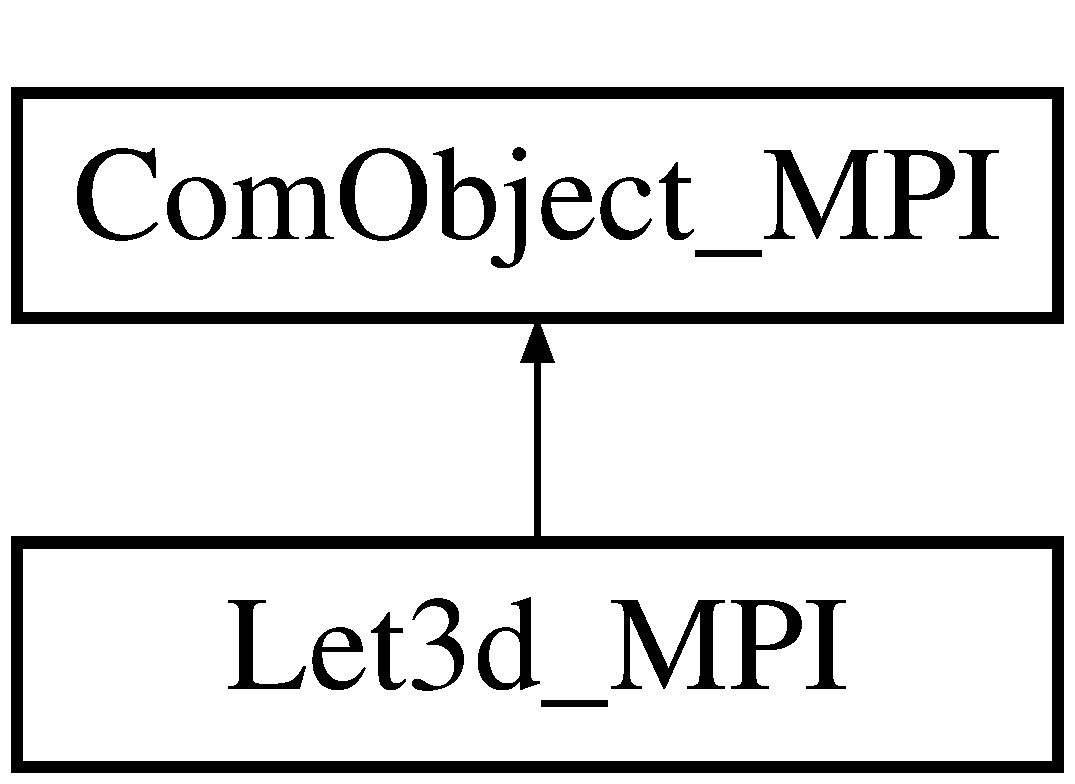
\includegraphics[height=2cm]{classLet3d__MPI}
\end{center}
\end{figure}


\subsection{Detailed Description}
LET = Local Essential Tree. See detailed description for more information. 

The LET is a global tree subset that a processor needs to evaluate the interaction on particles which belong to itself (owns). That is, it is a unique identifier: a set of points and its bounding box. To this extent, for a box/node B, the information from B's lists are needed. Specifically, the U, V, W and X lists are used for computation. More information is in the descriptiptions of \_\-Unodes, etc. and the papers. For a processor P, P's LET contains the boxes which P \char`\"{}owns\char`\"{} and boxes in the U,V,W and X lists of these boxes. For a box, B, owned by P, P is a contributor of B. If B is in the U,V,W or X lists of a box P owns, P is a user of B. For more information, see \char`\"{}A New Parallel Kernel-Independent Fast Multipole Method\char`\"{} by Ying, Biros, Zorin and Langston. 



Definition at line 51 of file let3d\_\-mpi.hpp.\subsection*{Public Member Functions}
\begin{CompactItemize}
\item 
{\bf Let3d\_\-MPI} (const string \&p)
\item 
{\bf $\sim$Let3d\_\-MPI} ()
\item 
Vec \& {\bf src\-Pos} ()
\item 
Vec \& {\bf trg\-Pos} ()
\item 
Point3 \& {\bf ctr} ()
\item 
int \& {\bf root\-Level} ()
\item 
double {\bf radius} ()
\item 
int \& {\bf pts\-Max} ()
\item 
int \& {\bf max\-Level} ()
\item 
int {\bf setup} ()
\item 
int {\bf print} ()
\item 
int {\bf src\-Data} ()
\item 
int {\bf trg\-Data} ()
\item 
int {\bf cal\-Glb\-Node\-Lists} (int g\-Node\-Idx)
\item 
int {\bf dwn\-Order\-Collect} (vector$<$ int $>$ \&)
\item 
int {\bf upw\-Order\-Collect} (vector$<$ int $>$ \&)
\item 
vector$<$ {\bf Node} $>$ \& {\bf node\-Vec} ()
\item 
{\bf Node} \& {\bf node} (int g\-Node\-Idx)
\item 
bool {\bf root} (int g\-Node\-Idx)
\item 
bool {\bf terminal} (int g\-Node\-Idx)
\item 
int {\bf parent} (int g\-Node\-Idx)
\item 
int {\bf child} (int g\-Node\-Idx, const Index3 \&Idx)
\item 
Index3 {\bf path2Node} (int g\-Node\-Idx)
\item 
int {\bf depth} (int g\-Node\-Idx)
\item 
Point3 {\bf center} (int g\-Node\-Idx)
\item 
double {\bf radius} (int g\-Node\-Idx)
\item 
int \& {\bf glb\-Glb\-Src\-Node\-Cnt} ()
\item 
int \& {\bf glb\-Glb\-Src\-Exa\-Cnt} ()
\item 
int \& {\bf lcl\-Glb\-Src\-Node\-Cnt} ()
\item 
int \& {\bf lcl\-Glb\-Src\-Exa\-Cnt} ()
\item 
int \& {\bf ctb\-Src\-Node\-Cnt} ()
\item 
int \& {\bf ctb\-Src\-Exa\-Cnt} ()
\item 
vector$<$ int $>$ \& {\bf ctb2Glb\-Src\-Node\-Map} ()
\item 
vector$<$ int $>$ \& {\bf ctb2Glb\-Src\-Exa\-Map} ()
\item 
int \& {\bf eva\-Trg\-Node\-Cnt} ()
\item 
int \& {\bf eva\-Trg\-Exa\-Cnt} ()
\item 
int \& {\bf usr\-Src\-Node\-Cnt} ()
\item 
int \& {\bf usr\-Src\-Exa\-Cnt} ()
\item 
vector$<$ int $>$ \& {\bf usr2Glb\-Src\-Node\-Map} ()
\item 
vector$<$ int $>$ \& {\bf usr2Glb\-Src\-Exa\-Map} ()
\item 
int {\bf find\-Glb\-Node} (int depth, const Index3 \&path2Node)
\item 
bool {\bf adjacent} (int me, int you)
\item 
int {\bf dim} () const 
\item 
int {\bf proc\-Lcl\-Num} (Vec pos)
\item 
int {\bf proc\-Glb\-Num} (Vec pos)
\item 
void {\bf proc\-Lcl\-Ran} (Vec pos, int \&beg, int \&end)
\end{CompactItemize}
\subsection*{Protected Attributes}
\begin{CompactItemize}
\item 
Vec {\bf \_\-src\-Pos}
\item 
Vec {\bf \_\-trg\-Pos}
\item 
Point3 {\bf \_\-ctr}
\item 
int {\bf \_\-root\-Level}
\item 
int {\bf \_\-pts\-Max}
\item 
int {\bf \_\-max\-Level}
\item 
vector$<$ {\bf Node} $>$ {\bf \_\-node\-Vec}
\item 
int {\bf \_\-glb\-Glb\-Src\-Node\-Cnt}
\item 
int {\bf \_\-glb\-Glb\-Src\-Exa\-Cnt}
\item 
int {\bf \_\-lcl\-Glb\-Src\-Node\-Cnt}
\item 
int {\bf \_\-lcl\-Glb\-Src\-Exa\-Cnt}
\item 
int {\bf \_\-ctb\-Src\-Node\-Cnt}
\item 
int {\bf \_\-ctb\-Src\-Exa\-Cnt}
\item 
vector$<$ int $>$ {\bf \_\-ctb2Glb\-Src\-Node\-Map}
\item 
vector$<$ int $>$ {\bf \_\-ctb2Glb\-Src\-Exa\-Map}
\item 
int {\bf \_\-eva\-Trg\-Node\-Cnt}
\item 
int {\bf \_\-eva\-Trg\-Exa\-Cnt}
\item 
int {\bf \_\-usr\-Src\-Node\-Cnt}
\item 
int {\bf \_\-usr\-Src\-Exa\-Cnt}
\item 
vector$<$ int $>$ {\bf \_\-usr2Glb\-Src\-Node\-Map}
\item 
vector$<$ int $>$ {\bf \_\-usr2Glb\-Src\-Exa\-Map}
\end{CompactItemize}
\subsection*{Classes}
\begin{CompactItemize}
\item 
class {\bf Node}
\begin{CompactList}\small\item\em The {\bf Node}{\rm (p.\,\pageref{classLet3d__MPI_1_1Node})} class stores information for a node or box in the octree. See for more detailed information. \item\end{CompactList}\item 
class {\bf Node\-Ext}
\begin{CompactList}\small\item\em {\bf Node\-Ext}{\rm (p.\,\pageref{classLet3d__MPI_1_1NodeExt})} stores information for a node such U, v, w, and X-lists as well as indices for contributor, evaluator and user nodes. \item\end{CompactList}\end{CompactItemize}


\subsection{Constructor \& Destructor Documentation}
\index{Let3d_MPI@{Let3d\_\-MPI}!Let3d_MPI@{Let3d\_\-MPI}}
\index{Let3d_MPI@{Let3d\_\-MPI}!Let3d_MPI@{Let3d\_\-MPI}}
\subsubsection{\setlength{\rightskip}{0pt plus 5cm}Let3d\_\-MPI::Let3d\_\-MPI (const string \& {\em p})}\label{classLet3d__MPI_0b17f9aae24c3678a5111a92d1b9ffb2_0b17f9aae24c3678a5111a92d1b9ffb2}


Construct Let3D\_\-MPI with string for Com\-Object 

Definition at line 29 of file let3d\_\-mpi.cpp.

\footnotesize\begin{verbatim}29                                    :
30   ComObject_MPI(p), _srcPos(NULL), _trgPos(NULL), _ctr(0.0), _rootLevel(0),
31   _ptsMax(150), _maxLevel(10)
32 {
33 }

\end{verbatim}\normalsize 


\index{Let3d_MPI@{Let3d\_\-MPI}!~Let3d_MPI@{$\sim$Let3d\_\-MPI}}
\index{~Let3d_MPI@{$\sim$Let3d\_\-MPI}!Let3d_MPI@{Let3d\_\-MPI}}
\subsubsection{\setlength{\rightskip}{0pt plus 5cm}Let3d\_\-MPI::$\sim$Let3d\_\-MPI ()}\label{classLet3d__MPI_ac2ccc7a2461eab6f090002aec2c87f9_ac2ccc7a2461eab6f090002aec2c87f9}




Definition at line 35 of file let3d\_\-mpi.cpp.

\footnotesize\begin{verbatim}36 {
37 }
\end{verbatim}\normalsize 




\subsection{Member Function Documentation}
\index{Let3d_MPI@{Let3d\_\-MPI}!adjacent@{adjacent}}
\index{adjacent@{adjacent}!Let3d_MPI@{Let3d\_\-MPI}}
\subsubsection{\setlength{\rightskip}{0pt plus 5cm}bool Let3d\_\-MPI::adjacent (int {\em me}, int {\em you})}\label{classLet3d__MPI_bd4b53389da8d68ee7218abbe006c28d_bd4b53389da8d68ee7218abbe006c28d}


Check if node\-Vec[me] is adjacent to node\-Vec[you] 

Definition at line 841 of file let3d\_\-mpi.cpp.

References \_\-\_\-FUNCT\_\-\_\-, depth(), path2Node(), and radius().

\footnotesize\begin{verbatim}842 {
843   int maxDepth = max(depth(me),depth(you)); /* Which node is at a greater depth */
844   Index3 one(1); /* = (1,1,1) */
845   /* Construct the center for both nodes */
846   Index3 meCtr(  (2*path2Node(me)+one) * pow2(maxDepth - depth(me))  );
847   Index3 youCtr(  (2*path2Node(you)+one) * pow2(maxDepth - depth(you))  );
848   /* construct radii for both nodes */
849   int meRad = pow2(maxDepth - depth(me));
850   int youRad = pow2(maxDepth - depth(you));
851   /* absolute value of difference of centers */
852   Index3 dif( abs(meCtr-youCtr) );
853   /* sum of radii */
854   int radius  = meRad + youRad;
855   /* if the abs. value of difference of centers is less than the sum of the radii
856         * AND the infinity norm equals the sum of the radii, then the two nodes
857         * are not too far away AND at least one edge touches */
858   return
859          ( dif <= Index3(radius) ) && //not too far
860          ( dif.linfty() == radius ); //at least one edge touch
861 }
\end{verbatim}\normalsize 


\index{Let3d_MPI@{Let3d\_\-MPI}!calGlbNodeLists@{calGlbNodeLists}}
\index{calGlbNodeLists@{calGlbNodeLists}!Let3d_MPI@{Let3d\_\-MPI}}
\subsubsection{\setlength{\rightskip}{0pt plus 5cm}int Let3d\_\-MPI::cal\-Glb\-Node\-Lists (int {\em g\-Node\-Idx})}\label{classLet3d__MPI_d1ba4ee8bb99cce06a89eb96cb9ddf8c_d1ba4ee8bb99cce06a89eb96cb9ddf8c}


Build U,V,W, and X lists for a specific node, indicated by an integer location in the global node index. 

Definition at line 635 of file let3d\_\-mpi.cpp.

\footnotesize\begin{verbatim}636 {
637   //begin
638   /* We use sets here since the values will be unnecessary to keep associated with the keys.
639         * Can also use a C++ map, but it is unnecessary here to maintain unique key/value pairs
640         * See let3d_mpi.hpp for descriptions of what U,B,W, and X lsists are. */
641   set<int> Uset, Vset, Wset, Xset;  
642   int curgNodeIdx = gNodeIdx;
643   /* Make sure current node is not the root as the root has no ancestors */
644   if(root(curgNodeIdx)==false) {
645          /* get parent of node we're interested in */
646          int pargNodeIdx = parent(curgNodeIdx);
647          Index3 minIdx(0); /* = (0,0,0) */
648          Index3 maxIdx(pow2(depth(curgNodeIdx))); /* = (2^d, 2^d, 2^d) */
649          
650          /* Try several different paths.  Here we are looking for paths which
651           * will lead to children of neighbors of the parent of the current node
652           * in order to build U,V,W, and X lists */
653          for(int i=-2; i<4; i++) {
654                 for(int j=-2; j<4; j++) {
655                   for(int k=-2; k<4; k++) {
656                          /* New Path to try */
657                          Index3 tryPath2Node( 2*path2Node(pargNodeIdx) + Index3(i,j,k) );
658                          /* Verify new path does not exceed a maximu index and is greater than (0,0,0) and is not equal to current node's path */
659                          if(tryPath2Node >= minIdx && tryPath2Node <  maxIdx && tryPath2Node != path2Node(curgNodeIdx)) {
660                                 /* Look for the children of the neighbors of the current node's parent */
661                                 int resgNodeIdx = findGlbNode(depth(curgNodeIdx), tryPath2Node);
662                                 /* adj = true if nodes have at least one edge touching */
663                                 bool adj = adjacent(resgNodeIdx, curgNodeIdx);
664                                 /* When test node is higher in the tree than current node */
665                                 if( depth(resgNodeIdx)<depth(curgNodeIdx) ) {
666                                   /* If adjacent and current node is a leaf, put test node in the Uset if the current node is a leaf */
667                                   if(adj){
668                                          if(terminal(curgNodeIdx)){ /* need to test if res a leaf?? HARPER */
669                                                 Uset.insert(resgNodeIdx);
670                                          }
671                                          else {;} /* non-leaves do not have U-lists */
672                                   }
673                                   else{
674                                          /* The nodes are not adjacent, but resgNodeIdx is still a child of the current node's parent's neighbors.
675                                           * Hence, the current node's parent is adjacent to resgNodeIdx.  IN general. the current node is in the
676                                           * W-list of resgNodeIdx */
677                                          Xset.insert(resgNodeIdx);
678                                   }
679                                 } /* End of "if depth(res) < depth(current) " */
680                                 
681                                 /* Current node and test node at same depth */
682                                 if( depth(resgNodeIdx)==depth(curgNodeIdx) ) {
683                                   /* Two nodes at same depth not adjacent */
684                                   if(!adj) {
685                                          Index3 bb(path2Node(resgNodeIdx)-path2Node(curgNodeIdx));
686                                          /* Verify that no single component of the two paths exceed a limit */
687                                          assert( bb.linfty()<=3 );
688                                          /* resgNodeIdx is a child of the neighbor's of the currentr node's parents and not-adjacent to current node.
689                                           * Hence, it is in the V-list */
690                                          Vset.insert(resgNodeIdx);
691                                   }
692                                   /* nodes at same depth and are adjacent, so resgNodeIdx could be in U OR W lists */
693                                   else {
694                                          if(terminal(curgNodeIdx)) {
695                                                 /* queue:  elements added/pushed to the back and removed/popped from the front */ 
696                                                 queue<int> rest;
697                                                 /* push resgNodeIdx into the queue */
698                                                 rest.push(resgNodeIdx);
699                                                 while(rest.empty()==false) {
700                                                   int fntgNodeIdx = rest.front(); rest.pop(); /* Set front temp node index and pop the list */
701                                                   /* If the current node and temp node are not adjacent, temp node is in W-list of current node */
702                                                   if(adjacent(fntgNodeIdx, curgNodeIdx)==false) {
703                                                          Wset.insert( fntgNodeIdx );
704                                                   }
705                                                   /* Current node and temp node ARE adjacent */
706                                                   else {
707                                                          /* If temp node is a leaf, it is in current node's U-list */
708                                                          if(terminal(fntgNodeIdx)) {
709                                                                 Uset.insert(fntgNodeIdx);
710                                                          }
711                                                          /* If temp node is not a leaf, then one of its descendants may be a leaf in the U or W lists of current node
712                                                          * So, we push those into the queue
713                                                          */
714                                                          else { 
715                                                                 for(int a=0; a<2; a++) {
716                                                                   for(int b=0; b<2; b++) {
717                                                                          for(int c=0; c<2; c++) {
718                                                                                 rest.push( child(fntgNodeIdx, Index3(a,b,c)) );
719                                                                          }
720                                                                   }
721                                                                 }
722                                                          }
723                                                   }
724                                                 } /* End of while loop for rest queue */
725                                          } /* End of "if current node a leaf" */ 
726                                   } /* End of res and current nodes at same depth and adjacent */
727                                 } /* End of "if depth(res) == depth(current)" */
728                          } /* End of trypath */
729                   }
730                 }
731          }
732   } /* End of building sets for non-root node, curgNodeIdx */
733 
734   /* If the current node is a leaf, then it is in its own U-list */
735   if(terminal(curgNodeIdx))
736          Uset.insert(curgNodeIdx);
737 
738   /* For all sets, check to make sure all of the nodes actually have sources in them.  If not
739         * we do not need to put them in the lists.  If so, build the U,V,W, and X lists from respective sets
740         */
741   for(set<int>::iterator si=Uset.begin(); si!=Uset.end(); si++)
742          if(node(*si).tag() & LET_SRCENODE) /* Check if sources bit set for this node's tag.  Same below */
743                 node(gNodeIdx).Unodes().push_back(*si);
744   for(set<int>::iterator si=Vset.begin(); si!=Vset.end(); si++)
745          if(node(*si).tag() & LET_SRCENODE)
746                 node(gNodeIdx).Vnodes().push_back(*si);
747   for(set<int>::iterator si=Wset.begin(); si!=Wset.end(); si++)
748          if(node(*si).tag() & LET_SRCENODE)
749                 node(gNodeIdx).Wnodes().push_back(*si);
750   for(set<int>::iterator si=Xset.begin(); si!=Xset.end(); si++)
751          if(node(*si).tag() & LET_SRCENODE)
752                 node(gNodeIdx).Xnodes().push_back(*si);
753   
754   return(0);
755 }
\end{verbatim}\normalsize 


\index{Let3d_MPI@{Let3d\_\-MPI}!center@{center}}
\index{center@{center}!Let3d_MPI@{Let3d\_\-MPI}}
\subsubsection{\setlength{\rightskip}{0pt plus 5cm}Point3 Let3d\_\-MPI::center (int {\em g\-Node\-Idx})}\label{classLet3d__MPI_dff5f922c11176af18f4bfa95c138a20_dff5f922c11176af18f4bfa95c138a20}


Return the center of the box dexcribed by node\-Vec[g\-Node\-Idx] 

Definition at line 793 of file let3d\_\-mpi.cpp.

\footnotesize\begin{verbatim}794 {
795   Point3 ll( ctr() - Point3(radius()) );
796   int tmp = pow2(depth(gNodeIdx));
797   Index3 path2Node_Lcl(path2Node(gNodeIdx));
798   Point3 res;
799   for(int d=0; d<dim(); d++) {
800          res(d) = ll(d) + (2*radius()) * (path2Node_Lcl(d)+0.5) / double(tmp);
801   }
802   return res;
803 }
\end{verbatim}\normalsize 


\index{Let3d_MPI@{Let3d\_\-MPI}!child@{child}}
\index{child@{child}!Let3d_MPI@{Let3d\_\-MPI}}
\subsubsection{\setlength{\rightskip}{0pt plus 5cm}int Let3d\_\-MPI::child (int {\em g\-Node\-Idx}, const Index3 \& {\em Idx})}\label{classLet3d__MPI_b0f154b8aff8346def992423c060b862_b0f154b8aff8346def992423c060b862}


Return child of node described by g\-Node\-Idx and Idx. g\-Node\-Idx is the Node's integer descriptor in node\-Vec and Idx is a binary index from 0-$>$7, indicating which child to return. For example, child(10,(0,0,0)) returns the first child of node\-Vec[10]. child(10,(1,1,1)) returns the eighth (and last) child of node\-Vec[10]. 

Definition at line 787 of file let3d\_\-mpi.cpp.

Referenced by find\-Glb\-Node().

\footnotesize\begin{verbatim}788 {
789   assert(idx>=Index3(0) && idx<Index3(2));
790   return node(gNodeIdx).chd() + (idx(0)*4+idx(1)*2+idx(2));
791 }
\end{verbatim}\normalsize 


\index{Let3d_MPI@{Let3d\_\-MPI}!ctb2GlbSrcExaMap@{ctb2GlbSrcExaMap}}
\index{ctb2GlbSrcExaMap@{ctb2GlbSrcExaMap}!Let3d_MPI@{Let3d\_\-MPI}}
\subsubsection{\setlength{\rightskip}{0pt plus 5cm}vector$<$int$>$\& Let3d\_\-MPI::ctb2Glb\-Src\-Exa\-Map ()\hspace{0.3cm}{\tt  [inline]}}\label{classLet3d__MPI_fa7b61748f05b09067f1fc99b672099e_fa7b61748f05b09067f1fc99b672099e}


Return vector of integers describing contributor to global exact source map 

Definition at line 338 of file let3d\_\-mpi.hpp.

References \_\-ctb2Glb\-Src\-Exa\-Map.

\footnotesize\begin{verbatim}338 { return _ctb2GlbSrcExaMap; }
\end{verbatim}\normalsize 


\index{Let3d_MPI@{Let3d\_\-MPI}!ctb2GlbSrcNodeMap@{ctb2GlbSrcNodeMap}}
\index{ctb2GlbSrcNodeMap@{ctb2GlbSrcNodeMap}!Let3d_MPI@{Let3d\_\-MPI}}
\subsubsection{\setlength{\rightskip}{0pt plus 5cm}vector$<$int$>$\& Let3d\_\-MPI::ctb2Glb\-Src\-Node\-Map ()\hspace{0.3cm}{\tt  [inline]}}\label{classLet3d__MPI_2edf7ec1048f348ac03b27bc90b9d2a0_2edf7ec1048f348ac03b27bc90b9d2a0}


Return vector of integers describing contributor to global source node map 

Definition at line 336 of file let3d\_\-mpi.hpp.

References \_\-ctb2Glb\-Src\-Node\-Map.

\footnotesize\begin{verbatim}336 { return _ctb2GlbSrcNodeMap; }
\end{verbatim}\normalsize 


\index{Let3d_MPI@{Let3d\_\-MPI}!ctbSrcExaCnt@{ctbSrcExaCnt}}
\index{ctbSrcExaCnt@{ctbSrcExaCnt}!Let3d_MPI@{Let3d\_\-MPI}}
\subsubsection{\setlength{\rightskip}{0pt plus 5cm}int\& Let3d\_\-MPI::ctb\-Src\-Exa\-Cnt ()\hspace{0.3cm}{\tt  [inline]}}\label{classLet3d__MPI_ef9a057fecc402d5d641067c9a43d7af_ef9a057fecc402d5d641067c9a43d7af}


Return exact count of contributor sources 

Definition at line 334 of file let3d\_\-mpi.hpp.

References \_\-ctb\-Src\-Exa\-Cnt.

\footnotesize\begin{verbatim}334 { return _ctbSrcExaCnt; }
\end{verbatim}\normalsize 


\index{Let3d_MPI@{Let3d\_\-MPI}!ctbSrcNodeCnt@{ctbSrcNodeCnt}}
\index{ctbSrcNodeCnt@{ctbSrcNodeCnt}!Let3d_MPI@{Let3d\_\-MPI}}
\subsubsection{\setlength{\rightskip}{0pt plus 5cm}int\& Let3d\_\-MPI::ctb\-Src\-Node\-Cnt ()\hspace{0.3cm}{\tt  [inline]}}\label{classLet3d__MPI_a558f7790d074c6bf0478d3d3300e595_a558f7790d074c6bf0478d3d3300e595}


Return number of contributor source nodes 

Definition at line 332 of file let3d\_\-mpi.hpp.

References \_\-ctb\-Src\-Node\-Cnt.

\footnotesize\begin{verbatim}332 { return _ctbSrcNodeCnt; }
\end{verbatim}\normalsize 


\index{Let3d_MPI@{Let3d\_\-MPI}!ctr@{ctr}}
\index{ctr@{ctr}!Let3d_MPI@{Let3d\_\-MPI}}
\subsubsection{\setlength{\rightskip}{0pt plus 5cm}Point3\& Let3d\_\-MPI::ctr ()\hspace{0.3cm}{\tt  [inline]}}\label{classLet3d__MPI_4b21bb4fef46b29bb3fb644f97b12415_4b21bb4fef46b29bb3fb644f97b12415}


Return center of tree 

Definition at line 257 of file let3d\_\-mpi.hpp.

References \_\-ctr.

Referenced by FMM3d\_\-MPI::setup().

\footnotesize\begin{verbatim}257 { return _ctr; }
\end{verbatim}\normalsize 


\index{Let3d_MPI@{Let3d\_\-MPI}!depth@{depth}}
\index{depth@{depth}!Let3d_MPI@{Let3d\_\-MPI}}
\subsubsection{\setlength{\rightskip}{0pt plus 5cm}int Let3d\_\-MPI::depth (int {\em g\-Node\-Idx})\hspace{0.3cm}{\tt  [inline]}}\label{classLet3d__MPI_365114de1453e803d05b02702d1e0bc2_365114de1453e803d05b02702d1e0bc2}


Return the depth in the octree of node\-Vec[g\-Node\-Idx] 

Definition at line 312 of file let3d\_\-mpi.hpp.

References Let3d\_\-MPI::Node::depth(), and node().

Referenced by adjacent(), find\-Glb\-Node(), and radius().

\footnotesize\begin{verbatim}312 { return node(gNodeIdx).depth(); }
\end{verbatim}\normalsize 


\index{Let3d_MPI@{Let3d\_\-MPI}!dim@{dim}}
\index{dim@{dim}!Let3d_MPI@{Let3d\_\-MPI}}
\subsubsection{\setlength{\rightskip}{0pt plus 5cm}int Let3d\_\-MPI::dim () const\hspace{0.3cm}{\tt  [inline]}}\label{classLet3d__MPI_3b54adb16617f4dccdd399f842f3f6bf_3b54adb16617f4dccdd399f842f3f6bf}


Return dimension. Always returns 3 

Definition at line 364 of file let3d\_\-mpi.hpp.

Referenced by proc\-Glb\-Num(), proc\-Lcl\-Num(), proc\-Lcl\-Ran(), and src\-Data().

\footnotesize\begin{verbatim}364 { return 3; }
\end{verbatim}\normalsize 


\index{Let3d_MPI@{Let3d\_\-MPI}!dwnOrderCollect@{dwnOrderCollect}}
\index{dwnOrderCollect@{dwnOrderCollect}!Let3d_MPI@{Let3d\_\-MPI}}
\subsubsection{\setlength{\rightskip}{0pt plus 5cm}int Let3d\_\-MPI::dwn\-Order\-Collect (vector$<$ int $>$ \&)}\label{classLet3d__MPI_1917ece529ea97f12e74e56e42b6d15a_1917ece529ea97f12e74e56e42b6d15a}


top down ordering of nodes 

Definition at line 759 of file let3d\_\-mpi.cpp.

References \_\-\_\-FUNCT\_\-\_\-.

\footnotesize\begin{verbatim}760 {
761   /* ordVec - ordering of the boxes in downward fashion */
762   ordVec.clear();
763   for(int i=0; i<_nodeVec.size(); i++)
764          ordVec.push_back(i);
765   return(0);
766 }
\end{verbatim}\normalsize 


\index{Let3d_MPI@{Let3d\_\-MPI}!evaTrgExaCnt@{evaTrgExaCnt}}
\index{evaTrgExaCnt@{evaTrgExaCnt}!Let3d_MPI@{Let3d\_\-MPI}}
\subsubsection{\setlength{\rightskip}{0pt plus 5cm}int\& Let3d\_\-MPI::eva\-Trg\-Exa\-Cnt ()\hspace{0.3cm}{\tt  [inline]}}\label{classLet3d__MPI_6d41ef754b4e311871e69d7b1056ba1c_6d41ef754b4e311871e69d7b1056ba1c}


Return exact count of evaluator sources 

Definition at line 343 of file let3d\_\-mpi.hpp.

References \_\-eva\-Trg\-Exa\-Cnt.

\footnotesize\begin{verbatim}343 { return _evaTrgExaCnt; }
\end{verbatim}\normalsize 


\index{Let3d_MPI@{Let3d\_\-MPI}!evaTrgNodeCnt@{evaTrgNodeCnt}}
\index{evaTrgNodeCnt@{evaTrgNodeCnt}!Let3d_MPI@{Let3d\_\-MPI}}
\subsubsection{\setlength{\rightskip}{0pt plus 5cm}int\& Let3d\_\-MPI::eva\-Trg\-Node\-Cnt ()\hspace{0.3cm}{\tt  [inline]}}\label{classLet3d__MPI_1999041d0ab14495560e04632d9b5707_1999041d0ab14495560e04632d9b5707}


Return number of evaluator source nodes 

Definition at line 341 of file let3d\_\-mpi.hpp.

References \_\-eva\-Trg\-Node\-Cnt.

\footnotesize\begin{verbatim}341 { return _evaTrgNodeCnt; }
\end{verbatim}\normalsize 


\index{Let3d_MPI@{Let3d\_\-MPI}!findGlbNode@{findGlbNode}}
\index{findGlbNode@{findGlbNode}!Let3d_MPI@{Let3d\_\-MPI}}
\subsubsection{\setlength{\rightskip}{0pt plus 5cm}int Let3d\_\-MPI::find\-Glb\-Node (int {\em depth}, const Index3 \& {\em path2Node})}\label{classLet3d__MPI_8ae25e5fad1314d14cedf18adc375fa3_8ae25e5fad1314d14cedf18adc375fa3}


Find a node in the global list based on a depth and path This is used for trying to find the children of the neighbors of the parent of some node at level \char`\"{}depth\char`\"{} for building that node's U,V,W, and X lists 

Definition at line 818 of file let3d\_\-mpi.cpp.

References child(), depth(), and terminal().

\footnotesize\begin{verbatim}819 {
820   int cur = 0;  
821   Index3 tmpPath2Node(wntPath2Node);
822   /* Keep trying to find a node cur which has depth greater than/equal to the given depth
823         * OR is a terminal/leaf */
824   while(depth(cur)<wntDepth && terminal(cur)==false) {
825          /* Difference in the depths */
826          int dif = wntDepth-depth(cur);
827          /* 2^(dif-1):  2^(difference in depths > 0) */
828          int tmp = pow2(dif-1);
829          /* Returns a binary index because of tmp's size */
830          Index3 choice( tmpPath2Node/tmp );
831 
832          /* Get new path to follow */
833          tmpPath2Node -= choice*tmp;
834          /* Choose new node - hopefully this node is at the same depth as our current node */
835          cur = child(cur, choice);       
836   }  //cerr<<endl;
837   return cur;
838 }
\end{verbatim}\normalsize 


\index{Let3d_MPI@{Let3d\_\-MPI}!glbGlbSrcExaCnt@{glbGlbSrcExaCnt}}
\index{glbGlbSrcExaCnt@{glbGlbSrcExaCnt}!Let3d_MPI@{Let3d\_\-MPI}}
\subsubsection{\setlength{\rightskip}{0pt plus 5cm}int\& Let3d\_\-MPI::glb\-Glb\-Src\-Exa\-Cnt ()\hspace{0.3cm}{\tt  [inline]}}\label{classLet3d__MPI_1d4278c762704adf15862ec5554f846c_1d4278c762704adf15862ec5554f846c}


Return global exact number of sources, available to all processors 

Definition at line 325 of file let3d\_\-mpi.hpp.

References \_\-glb\-Glb\-Src\-Exa\-Cnt.

\footnotesize\begin{verbatim}325 { return _glbGlbSrcExaCnt; }
\end{verbatim}\normalsize 


\index{Let3d_MPI@{Let3d\_\-MPI}!glbGlbSrcNodeCnt@{glbGlbSrcNodeCnt}}
\index{glbGlbSrcNodeCnt@{glbGlbSrcNodeCnt}!Let3d_MPI@{Let3d\_\-MPI}}
\subsubsection{\setlength{\rightskip}{0pt plus 5cm}int\& Let3d\_\-MPI::glb\-Glb\-Src\-Node\-Cnt ()\hspace{0.3cm}{\tt  [inline]}}\label{classLet3d__MPI_1cd7d83fe77fb464b606265d4f31c050_1cd7d83fe77fb464b606265d4f31c050}


Return global source node count, available to all processors 

Definition at line 323 of file let3d\_\-mpi.hpp.

References \_\-glb\-Glb\-Src\-Node\-Cnt.

\footnotesize\begin{verbatim}323 { return _glbGlbSrcNodeCnt; }
\end{verbatim}\normalsize 


\index{Let3d_MPI@{Let3d\_\-MPI}!lclGlbSrcExaCnt@{lclGlbSrcExaCnt}}
\index{lclGlbSrcExaCnt@{lclGlbSrcExaCnt}!Let3d_MPI@{Let3d\_\-MPI}}
\subsubsection{\setlength{\rightskip}{0pt plus 5cm}int\& Let3d\_\-MPI::lcl\-Glb\-Src\-Exa\-Cnt ()\hspace{0.3cm}{\tt  [inline]}}\label{classLet3d__MPI_c059775b0357cf1bff1dec7bcfb8bd33_c059775b0357cf1bff1dec7bcfb8bd33}


Return local exact number of sources 

Definition at line 329 of file let3d\_\-mpi.hpp.

References \_\-lcl\-Glb\-Src\-Exa\-Cnt.

\footnotesize\begin{verbatim}329 { return _lclGlbSrcExaCnt; }
\end{verbatim}\normalsize 


\index{Let3d_MPI@{Let3d\_\-MPI}!lclGlbSrcNodeCnt@{lclGlbSrcNodeCnt}}
\index{lclGlbSrcNodeCnt@{lclGlbSrcNodeCnt}!Let3d_MPI@{Let3d\_\-MPI}}
\subsubsection{\setlength{\rightskip}{0pt plus 5cm}int\& Let3d\_\-MPI::lcl\-Glb\-Src\-Node\-Cnt ()\hspace{0.3cm}{\tt  [inline]}}\label{classLet3d__MPI_52319021e6ad3f34cc15791c10d29672_52319021e6ad3f34cc15791c10d29672}


Return local source node count 

Definition at line 327 of file let3d\_\-mpi.hpp.

References \_\-lcl\-Glb\-Src\-Node\-Cnt.

\footnotesize\begin{verbatim}327 { return _lclGlbSrcNodeCnt; }
\end{verbatim}\normalsize 


\index{Let3d_MPI@{Let3d\_\-MPI}!maxLevel@{maxLevel}}
\index{maxLevel@{maxLevel}!Let3d_MPI@{Let3d\_\-MPI}}
\subsubsection{\setlength{\rightskip}{0pt plus 5cm}int\& Let3d\_\-MPI::max\-Level ()\hspace{0.3cm}{\tt  [inline]}}\label{classLet3d__MPI_fdc3ca03e415e2d7b0b1f708d3ab94bb_fdc3ca03e415e2d7b0b1f708d3ab94bb}


Return maximum number of levels in tree 

Definition at line 265 of file let3d\_\-mpi.hpp.

References \_\-max\-Level.

\footnotesize\begin{verbatim}265 { return _maxLevel; }
\end{verbatim}\normalsize 


\index{Let3d_MPI@{Let3d\_\-MPI}!node@{node}}
\index{node@{node}!Let3d_MPI@{Let3d\_\-MPI}}
\subsubsection{\setlength{\rightskip}{0pt plus 5cm}{\bf Node}\& Let3d\_\-MPI::node (int {\em g\-Node\-Idx})\hspace{0.3cm}{\tt  [inline]}}\label{classLet3d__MPI_f259ccf218dbf0a04530841785f1a8b0_f259ccf218dbf0a04530841785f1a8b0}


Return a specific node in node\-Vec using an integer locater. I.e., \_\-node\-Vec[g\-Node\-Idx] 

Definition at line 293 of file let3d\_\-mpi.hpp.

References \_\-node\-Vec.

Referenced by FMM3d\_\-MPI::ctb\-Src\-Exa\-Den(), FMM3d\_\-MPI::ctb\-Src\-Exa\-Nor(), FMM3d\_\-MPI::ctb\-Src\-Upw\-Chk\-Val(), FMM3d\_\-MPI::ctb\-Src\-Upw\-Equ\-Den(), depth(), FMM3d\_\-MPI::evaluate(), FMM3d\_\-MPI::eva\-Trg\-Dwn\-Chk\-Val(), FMM3d\_\-MPI::eva\-Trg\-Dwn\-Equ\-Den(), FMM3d\_\-MPI::eva\-Trg\-Exa\-Pos(), FMM3d\_\-MPI::eva\-Trg\-Exa\-Val(), parent(), path2Node(), root(), terminal(), FMM3d\_\-MPI::usr\-Src\-Exa\-Den(), FMM3d\_\-MPI::usr\-Src\-Exa\-Nor(), FMM3d\_\-MPI::usr\-Src\-Exa\-Pos(), and FMM3d\_\-MPI::usr\-Src\-Upw\-Equ\-Den().

\footnotesize\begin{verbatim}293 { return _nodeVec[gNodeIdx]; }
\end{verbatim}\normalsize 


\index{Let3d_MPI@{Let3d\_\-MPI}!nodeVec@{nodeVec}}
\index{nodeVec@{nodeVec}!Let3d_MPI@{Let3d\_\-MPI}}
\subsubsection{\setlength{\rightskip}{0pt plus 5cm}vector$<${\bf Node}$>$\& Let3d\_\-MPI::node\-Vec ()\hspace{0.3cm}{\tt  [inline]}}\label{classLet3d__MPI_44c0c8da466878274feb4ce060c10b9b_44c0c8da466878274feb4ce060c10b9b}


Return the vector of Nodes 

Definition at line 291 of file let3d\_\-mpi.hpp.

References \_\-node\-Vec.

\footnotesize\begin{verbatim}291 { return _nodeVec; }
\end{verbatim}\normalsize 


\index{Let3d_MPI@{Let3d\_\-MPI}!parent@{parent}}
\index{parent@{parent}!Let3d_MPI@{Let3d\_\-MPI}}
\subsubsection{\setlength{\rightskip}{0pt plus 5cm}int Let3d\_\-MPI::parent (int {\em g\-Node\-Idx})\hspace{0.3cm}{\tt  [inline]}}\label{classLet3d__MPI_eedcae6652a6a95ae0ef366d7e8ad0ef_eedcae6652a6a95ae0ef366d7e8ad0ef}


Return the integer locater (in node\-Vec) of the parent of a node 

Definition at line 299 of file let3d\_\-mpi.hpp.

References node(), and Let3d\_\-MPI::Node::par().

\footnotesize\begin{verbatim}299 { assert(node(gNodeIdx).par()!=-1); return node(gNodeIdx).par(); }
\end{verbatim}\normalsize 


\index{Let3d_MPI@{Let3d\_\-MPI}!path2Node@{path2Node}}
\index{path2Node@{path2Node}!Let3d_MPI@{Let3d\_\-MPI}}
\subsubsection{\setlength{\rightskip}{0pt plus 5cm}Index3 Let3d\_\-MPI::path2Node (int {\em g\-Node\-Idx})\hspace{0.3cm}{\tt  [inline]}}\label{classLet3d__MPI_8df44bec9d337d228d001b12e5e6379e_8df44bec9d337d228d001b12e5e6379e}


Return an Index3 which gives a binary descriptor of the path to the node at node\-Vec[g\-Node\-Idx] The integer vector (x,y,z) and its binary expansion tells how to go from the root box to the current box (0 stands for up/left and 1 for bottom/down, etc.). 

Definition at line 310 of file let3d\_\-mpi.hpp.

References node(), and Let3d\_\-MPI::Node::path2Node().

Referenced by adjacent().

\footnotesize\begin{verbatim}310 { return node(gNodeIdx).path2Node(); }
\end{verbatim}\normalsize 


\index{Let3d_MPI@{Let3d\_\-MPI}!print@{print}}
\index{print@{print}!Let3d_MPI@{Let3d\_\-MPI}}
\subsubsection{\setlength{\rightskip}{0pt plus 5cm}int Let3d\_\-MPI::print ()}\label{classLet3d__MPI_d0d33c63402dfb2c02713a7fd52578c1_d0d33c63402dfb2c02713a7fd52578c1}


Print out information: Petsc\-Printf(MPI\_\-COMM\_\-SELF, \char`\"{}\%d: \%d glb\-Glb\-Src \%d \%d  lcl\-Glb\-Src \%d \%d ctb\-Src \%d \%d eva\-Trg \%d \%d usr\-Src \%d \%d$\backslash$n\char`\"{}, {\bf mpi\-Rank()}{\rm (p.\,\pageref{classComObject__MPI_ae51fcdfaec9ca26c842280cf6b99aa9_ae51fcdfaec9ca26c842280cf6b99aa9})}, \_\-node\-Vec.size(),\_\-glb\-Glb\-Src\-Node\-Cnt, \_\-glb\-Glb\-Src\-Exa\-Cnt, \_\-lcl\-Glb\-Src\-Node\-Cnt, \_\-lcl\-Glb\-Src\-Exa\-Cnt, \_\-ctb\-Src\-Node\-Cnt, \_\-ctb\-Src\-Exa\-Cnt, \_\-eva\-Trg\-Node\-Cnt, \_\-eva\-Trg\-Exa\-Cnt, \_\-usr\-Src\-Node\-Cnt, \_\-usr\-Src\-Exa\-Cnt) ); 

Definition at line 866 of file let3d\_\-mpi.cpp.

References \_\-ctb\-Src\-Exa\-Cnt, \_\-ctb\-Src\-Node\-Cnt, \_\-eva\-Trg\-Exa\-Cnt, \_\-eva\-Trg\-Node\-Cnt, \_\-glb\-Glb\-Src\-Exa\-Cnt, \_\-glb\-Glb\-Src\-Node\-Cnt, \_\-lcl\-Glb\-Src\-Exa\-Cnt, \_\-lcl\-Glb\-Src\-Node\-Cnt, \_\-node\-Vec, \_\-usr\-Src\-Exa\-Cnt, \_\-usr\-Src\-Node\-Cnt, Com\-Object\_\-MPI::mpi\-Rank(), and p\-C.

\footnotesize\begin{verbatim}867 {
868   //begin  //pC( PetscPrintf(MPI_COMM_WORLD, "nodeVec %d\n", _nodeVec.size()) );
869   pC( PetscPrintf(MPI_COMM_SELF, "%d: %d glbGlbSrc %d %d  lclGlbSrc %d %d ctbSrc %d %d evaTrg %d %d usrSrc %d %d\n",
870                                                 mpiRank(), _nodeVec.size(),
871                                                 _glbGlbSrcNodeCnt, _glbGlbSrcExaCnt,   _lclGlbSrcNodeCnt, _lclGlbSrcExaCnt,
872                                                 _ctbSrcNodeCnt, _ctbSrcExaCnt,   _evaTrgNodeCnt, _evaTrgExaCnt,                 _usrSrcNodeCnt, _usrSrcExaCnt) );
873   return(0);
874 }
\end{verbatim}\normalsize 


\index{Let3d_MPI@{Let3d\_\-MPI}!procGlbNum@{procGlbNum}}
\index{procGlbNum@{procGlbNum}!Let3d_MPI@{Let3d\_\-MPI}}
\subsubsection{\setlength{\rightskip}{0pt plus 5cm}int Let3d\_\-MPI::proc\-Glb\-Num (Vec {\em pos})\hspace{0.3cm}{\tt  [inline]}}\label{classLet3d__MPI_47cb2afea618c56a5cc6e05f4034a806_47cb2afea618c56a5cc6e05f4034a806}


For a certain processor, return global number of positions from Vec pos 

Definition at line 370 of file let3d\_\-mpi.hpp.

References dim().

\footnotesize\begin{verbatim}370 { int tmp; VecGetSize(     pos, &tmp); return tmp/dim(); }
\end{verbatim}\normalsize 


\index{Let3d_MPI@{Let3d\_\-MPI}!procLclNum@{procLclNum}}
\index{procLclNum@{procLclNum}!Let3d_MPI@{Let3d\_\-MPI}}
\subsubsection{\setlength{\rightskip}{0pt plus 5cm}int Let3d\_\-MPI::proc\-Lcl\-Num (Vec {\em pos})\hspace{0.3cm}{\tt  [inline]}}\label{classLet3d__MPI_21f80b863e1376ff6648d882fdabd08e_21f80b863e1376ff6648d882fdabd08e}


For a certain processor, return local number of positions from Vec pos See {\tt http://www-unix.mcs.anl.gov/petsc/petsc-as/snapshots/petsc-current/docs/manualpages/Vec/Vec\-Get\-Local\-Size.html} for more info 

Definition at line 368 of file let3d\_\-mpi.hpp.

References dim().

Referenced by src\-Data().

\footnotesize\begin{verbatim}368 { int tmp; VecGetLocalSize(pos, &tmp); return tmp/dim(); }
\end{verbatim}\normalsize 


\index{Let3d_MPI@{Let3d\_\-MPI}!procLclRan@{procLclRan}}
\index{procLclRan@{procLclRan}!Let3d_MPI@{Let3d\_\-MPI}}
\subsubsection{\setlength{\rightskip}{0pt plus 5cm}void Let3d\_\-MPI::proc\-Lcl\-Ran (Vec {\em pos}, int \& {\em beg}, int \& {\em end})\hspace{0.3cm}{\tt  [inline]}}\label{classLet3d__MPI_c77ddf71aecd48cd8a8ed887d5bcd834_c77ddf71aecd48cd8a8ed887d5bcd834}


For a certain preocessor, return local range in beg and end for Vec pos of the local ownership See {\tt http://www-unix.mcs.anl.gov/petsc/petsc-as/snapshots/petsc-current/docs/manualpages/Vec/Vec\-Get\-Ownership\-Range.html} for more information 

Definition at line 373 of file let3d\_\-mpi.hpp.

References dim().

Referenced by FMM3d\_\-MPI::evaluate().

\footnotesize\begin{verbatim}373 { VecGetOwnershipRange(pos, &beg, &end); beg=beg/dim(); end=end/dim(); }
\end{verbatim}\normalsize 


\index{Let3d_MPI@{Let3d\_\-MPI}!ptsMax@{ptsMax}}
\index{ptsMax@{ptsMax}!Let3d_MPI@{Let3d\_\-MPI}}
\subsubsection{\setlength{\rightskip}{0pt plus 5cm}int\& Let3d\_\-MPI::pts\-Max ()\hspace{0.3cm}{\tt  [inline]}}\label{classLet3d__MPI_682c29880d87862bd529f951970bf83a_682c29880d87862bd529f951970bf83a}


Return maximum number of points, set during setup from options file 

Definition at line 263 of file let3d\_\-mpi.hpp.

References \_\-pts\-Max.

\footnotesize\begin{verbatim}263 { return _ptsMax; }
\end{verbatim}\normalsize 


\index{Let3d_MPI@{Let3d\_\-MPI}!radius@{radius}}
\index{radius@{radius}!Let3d_MPI@{Let3d\_\-MPI}}
\subsubsection{\setlength{\rightskip}{0pt plus 5cm}double Let3d\_\-MPI::radius (int {\em g\-Node\-Idx})}\label{classLet3d__MPI_c1534d5f7ba6030886668befb2b472c0_c1534d5f7ba6030886668befb2b472c0}


Return the radius of node\-Vec[g\-Node\-Idx]: That is, the radius of the root divide by 2$^\wedge$(depth of the node at g\-Node\-Ix) If the root\-Level is zero, then {\bf radius()}{\rm (p.\,\pageref{classLet3d__MPI_703550342372334b492a37f2f4379409_703550342372334b492a37f2f4379409})} is one, such that radius(i) = 1/(2$^\wedge$(depth(i))) 

Definition at line 809 of file let3d\_\-mpi.cpp.

References depth(), and radius().

\footnotesize\begin{verbatim}810 {
811   return radius()/double(pow2(depth(gNodeIdx)));
812 }
\end{verbatim}\normalsize 


\index{Let3d_MPI@{Let3d\_\-MPI}!radius@{radius}}
\index{radius@{radius}!Let3d_MPI@{Let3d\_\-MPI}}
\subsubsection{\setlength{\rightskip}{0pt plus 5cm}double Let3d\_\-MPI::radius ()\hspace{0.3cm}{\tt  [inline]}}\label{classLet3d__MPI_703550342372334b492a37f2f4379409_703550342372334b492a37f2f4379409}


return root's radius (2$^\wedge$(-root\-Level)) 

Definition at line 261 of file let3d\_\-mpi.hpp.

References \_\-root\-Level.

Referenced by adjacent(), and radius().

\footnotesize\begin{verbatim}261 { return pow(2.0, -_rootLevel); }
\end{verbatim}\normalsize 


\index{Let3d_MPI@{Let3d\_\-MPI}!root@{root}}
\index{root@{root}!Let3d_MPI@{Let3d\_\-MPI}}
\subsubsection{\setlength{\rightskip}{0pt plus 5cm}bool Let3d\_\-MPI::root (int {\em g\-Node\-Idx})\hspace{0.3cm}{\tt  [inline]}}\label{classLet3d__MPI_06ef4c5a5a60303ba9b0b041a8bb5000_06ef4c5a5a60303ba9b0b041a8bb5000}


If a node has no parent, then it is the root 

Definition at line 295 of file let3d\_\-mpi.hpp.

References node(), and Let3d\_\-MPI::Node::par().

\footnotesize\begin{verbatim}295 { return node(gNodeIdx).par()==-1; }
\end{verbatim}\normalsize 


\index{Let3d_MPI@{Let3d\_\-MPI}!rootLevel@{rootLevel}}
\index{rootLevel@{rootLevel}!Let3d_MPI@{Let3d\_\-MPI}}
\subsubsection{\setlength{\rightskip}{0pt plus 5cm}int\& Let3d\_\-MPI::root\-Level ()\hspace{0.3cm}{\tt  [inline]}}\label{classLet3d__MPI_f80fcb36cb42936f1912fe8c85ec96e4_f80fcb36cb42936f1912fe8c85ec96e4}


Return root level (usually zero or one) 

Definition at line 259 of file let3d\_\-mpi.hpp.

References \_\-root\-Level.

Referenced by FMM3d\_\-MPI::setup().

\footnotesize\begin{verbatim}259 { return _rootLevel; }
\end{verbatim}\normalsize 


\index{Let3d_MPI@{Let3d\_\-MPI}!setup@{setup}}
\index{setup@{setup}!Let3d_MPI@{Let3d\_\-MPI}}
\subsubsection{\setlength{\rightskip}{0pt plus 5cm}int Let3d\_\-MPI::setup ()}\label{classLet3d__MPI_415266b005d267e801176f27c0434a50_415266b005d267e801176f27c0434a50}


setup function. gets ptx\-Max and max\-Level as well as runs {\bf src\-Data()}{\rm (p.\,\pageref{classLet3d__MPI_44ef9057a3adc0372c2569c172064dac_44ef9057a3adc0372c2569c172064dac})} and {\bf trg\-Data()}{\rm (p.\,\pageref{classLet3d__MPI_ca481263feff458d83769363d3ad85f7_ca481263feff458d83769363d3ad85f7})} for construction 

Definition at line 43 of file let3d\_\-mpi.cpp.

References \_\-\_\-FUNCT\_\-\_\-, \_\-max\-Level, \_\-pts\-Max, p\-A, p\-C, Com\-Object\_\-MPI::prefix(), src\-Data(), and trg\-Data().

Referenced by FMM3d\_\-MPI::setup().

\footnotesize\begin{verbatim}44 {
45   //begin
46   //--------
47   PetscTruth flg = PETSC_FALSE;
48   /* Get the maximum number of points per leaf level box and max number of levels in the tree */
49   pC( PetscOptionsGetInt( prefix().c_str(), "-ptsMax",   &_ptsMax,   &flg) ); pA(flg==true);
50   pC( PetscOptionsGetInt( prefix().c_str(), "-maxLevel", &_maxLevel, &flg) ); pA(flg==true);
51   //--------
52   pC( srcData() );  
53   pC( trgData() );  
54   return(0);
55 }
\end{verbatim}\normalsize 


\index{Let3d_MPI@{Let3d\_\-MPI}!srcData@{srcData}}
\index{srcData@{srcData}!Let3d_MPI@{Let3d\_\-MPI}}
\subsubsection{\setlength{\rightskip}{0pt plus 5cm}int Let3d\_\-MPI::src\-Data ()}\label{classLet3d__MPI_44ef9057a3adc0372c2569c172064dac_44ef9057a3adc0372c2569c172064dac}


Assign all of the source data as necessary as well as set necessary variables for sources. See {\bf let3d\_\-mpi.cpp}{\rm (p.\,\pageref{let3d__mpi_8cpp})} for more information 

Definition at line 64 of file let3d\_\-mpi.cpp.

References \_\-src\-Pos, dim(), p\-A, p\-C, and proc\-Lcl\-Num().

Referenced by setup().

\footnotesize\begin{verbatim}65 {
66   /* Set the sample DENSITY to 1/10 th of the original positions */
67   double DENSITY = 1.0/10.0;
68   
69   /* sample data with density - local sample positions vector */
70   vector<Point3> lclSamPosVec;
71   {
72          Vec pos = _srcPos;
73     double* posArr; pC( VecGetArray(pos, &posArr) );
74          /* number of local positions for this processor */
75          int numLclPos = procLclNum(pos);
76          /* number of local sample positions for this processor */
77          int numLclSamPos = int(ceil(procLclNum(pos) * DENSITY));
78          /* sample a fraction of the original sources and
79           * store these points in lclSamPosVec - local sample positions vector */
80          for(int k=0; k<numLclSamPos; k++) {
81                 int tmpIdx = int(floor(drand48() * numLclPos));
82                 Point3 tmppt(posArr + tmpIdx*dim());
83                 lclSamPosVec.push_back( tmppt );
84          }
85          pA(lclSamPosVec.size()==numLclSamPos); /* Verify that the local sample positions vector is the size we want */
86          pC( VecRestoreArray(pos, &posArr) ); /* Restore the full global vector of positions */
87   } /* end of this scope - psArr, numLclcPos, numLclSamPos, pos no longer available */
88 
89   
90   
91   /* all procs send sample positions to proc 0 */
92   vector<Point3> allSamPosVec; /* will store all sample positions for all processors */
93   {
94          int numLcl = lclSamPosVec.size(); /* number = numLclSamPos */
95          int sizLcl = numLcl * dim(); /* local size = number of local sample positions times the dimension (3) */
96 
97          /* vector storing size of local vectors.  i.e., if mpisize()==2
98           * sizLclVec is a vector of length 2, where sizLclVec[i] stores the
99           * number of sample positions at the processor of rank i */
100          vector<int> sizLclVec(mpiSize()); 
101          /* MPI_Gather information:  http://www-unix.mcs.anl.gov/mpi/www/www3/MPI_Gather.html
102          * Here, we're gathering all sizLcl values at the buffer located in memory at &(sizLclVec[0]) onr int at a time */
103          pC( MPI_Gather(&sizLcl, 1, MPI_INT, &(sizLclVec[0]), 1, MPI_INT, 0, mpiComm()) );
104          
105          int sizGlb = 0; /* sizGlb will collect all sizLcl values */
106          for(int i=0; i<sizLclVec.size(); i++){
107                 sizGlb += sizLclVec[i];
108          }
109          /* number of global sample positions for all processors */
110          int numGlb = sizGlb / dim(); 
111          /* displacement global vector - tells how far into allSamPosVec need to go to get to processor i's samples */
112          vector<int> disGlbVec(mpiSize()); 
113          int cnt = 0;
114          for(int i=0; i<sizLclVec.size(); i++) {
115                 disGlbVec[i] = cnt;
116                 cnt += sizLclVec[i];     }
117          pA(cnt==sizGlb);
118          
119          if(mpiRank()==0)               allSamPosVec.resize(numGlb); /* allSamPosVec stores numGlb points of type Point3 */
120          /* Information on MPI_Gatherv http://www-unix.mcs.anl.gov/mpi/www/www3/MPI_Gatherv.html
121          * Like MPI_Gather - all lclSamPosVec points are sent to the allSamPosVec vector.  sizLclVec[i] and disGlbVec[i] will
122          * indicate how to navigate allSamPosVec for processor i */
123          pC( MPI_Gatherv(&(lclSamPosVec[0]), sizLcl, MPI_DOUBLE, &(allSamPosVec[0]), &(sizLclVec[0]), &(disGlbVec[0]), MPI_DOUBLE, 0, mpiComm()) );
124          
125          lclSamPosVec.clear();
126   } /* end of this scope - sizLclcVec and disGlbVec no longer available */
127   
128   /* processor 0  builds the tree 
129         * The tree is build based on sample positions since we will
130         * have a max number of points per box.  Sampling positions for
131         * LET building makes the build faster */
132   vector<Node>& nodeVec = this->nodeVec(); nodeVec.clear();
133   if(mpiRank()==0) {
134          /* vector of vector of indices */
135          vector< vector<int> > vecIdxs;
136          /* local source number - number of source points in each box */
137          vector<int> lclSrcNumVec;
138 
139          /* Push the root node.  No parent or child, path2Node = (0,0,0), depth 0 */
140          nodeVec.push_back( Node(-1,-1,Index3(0,0,0), 0) );
141          vecIdxs.push_back( vector<int>() );
142          /* vecIdxs[0] will store all indices put into curVecIdxs */
143          vector<int>& curVecIdxs = vecIdxs[0];
144          Point3 bbmin(ctr()-Point3(radius()));
145          Point3 bbmax(ctr()+Point3(radius()));
146          /* For all sample points, make sure that it is within the root's radius distance from the center of the tree */
147          for(int k=0; k<allSamPosVec.size(); k++) {
148                 Point3 tmp(allSamPosVec[k]);
149                 /* Assertion kills implementation at runtime of point not within prescribed box */
150                 pA( tmp>=bbmin && tmp<=bbmax );
151                 curVecIdxs.push_back(k);
152          }
153          /* the local number of sources vector stores the size of all sample points in the 0 position for the root */
154          lclSrcNumVec.push_back( curVecIdxs.size() );
155 
156          /* Sample points max number of points per leaf box */
157          int PTSMAX = (int)ceil(ptsMax() * DENSITY);
158          
159          int level = 0;
160          int arrBeg = 0;
161          int arrEnd = 1;
162          while(arrBeg < arrEnd) {
163                 int arrCnt = arrEnd;
164                 /* In this for loop, we build each level as necessary
165                 * arrBeg will be set to the number of points already parsed after this for loop*/
166                 for(int k=arrBeg; k<arrEnd; k++) {
167                   //--
168                   /* lclSrcNumVec[0] is already set to the size of all of the sample positions within radius of the center
169                   * So, lclSrcNumVec[k] at each level is set such that the maximum number of points is in the subsequent
170                   * children boxes at a maximum level */
171                   if( lclSrcNumVec[k]>PTSMAX && level<maxLevel()-1) {
172                          /* the current node's child locator is set to arrCnt (the number of boxes already built)
173                           * For example, when k = 0, arrCnt = 1.  The location of the root's lead child */
174                          nodeVec[k].chd() = arrCnt;
175                          /* Increment arrCnt by 8 */
176                          arrCnt = arrCnt + pow2(dim());
177                          /* Build all 8 of nodeVec[k]'s children */
178                          for(int a=0; a<2; a++) {
179                                 for(int b=0; b<2; b++) {
180                                   for(int c=0; c<2; c++) {
181                                          /* Create a new node with parent at location "k"
182                                           * child initially set to -1 (changed when new node is looked at)
183                                           * path set to 2*"k's path" + the binary index of the new node's location relative to k
184                                           * depth is set to "k's" depth + 1
185                                           */
186                                          nodeVec.push_back( Node(k,-1, 2*nodeVec[k].path2Node()+Index3(a,b,c), nodeVec[k].depth()+1) );
187                                          /* push a new vector of integers onto vecIdxs */
188                                          vecIdxs.push_back( vector<int>() );
189                                          /* Push an extra level onto lclSrcNumVec - set to zero for now and will be changed later */
190                                          lclSrcNumVec.push_back( 0 );
191                                   }
192                                 }
193                          }
194                          /* children's vector of indices */ 
195                          Point3 curctr( center(k) ); /* get center of current node */
196                          /* vecIdxs[k] stores indices of sample points that node k has in it
197                           * for vecIdxs[0], all of the sample points indices are stored */
198                          for(vector<int>::iterator pi=vecIdxs[k].begin(); pi!=vecIdxs[k].end(); pi++) {
199                                 /* Build a point out of the index *pi which is in the current node's vector of indices */
200                                 Point3 tmp( allSamPosVec[*pi] );
201                                 Index3 idx;
202                                 /* Build an index based on the point tmp's location relative to the center of the node k */
203                                 for(int j=0; j<dim(); j++)
204                                   idx(j) = (tmp(j) >= curctr(j));
205                                 /* return the index of the child of node k located at idx */
206                                 int chdgNodeIdx = child(k, idx);
207                                 /* put the point references by *pi into the index of points that the node at chgNodeIdx has access to */
208                                 vecIdxs[chdgNodeIdx].push_back(*pi);
209                          }
210                          vecIdxs[k].clear(); //VERY IMPORTANT
211                          /* children's lclSrcNum */
212                          for(int a=0; a<2; a++) {
213                                 for(int b=0; b<2; b++) {
214                                   for(int c=0; c<2; c++) {
215                                          int chdgNodeIdx = child( k, Index3(a,b,c) );
216                                          /* the local number of sources for the node at chdgNodeIdx is the size of its vector of indices */
217                                          lclSrcNumVec[chdgNodeIdx] = vecIdxs[chdgNodeIdx].size();
218                                   }
219                                 } 
220                          }
221                   } /* end of if */
222                 } /* end of for */
223                 /* the previous level has been built so increment the levels and update arr counters */
224                 level++;
225                 arrBeg = arrEnd;
226                 arrEnd = arrCnt;
227          } /* end of while */
228          
229          allSamPosVec.clear(); //SAVE SPACE
230   } /* End of building the tree on processor zero */
231   /* end of this scope.  everything in this scope, including lclSrcNumVec and vecIdxs no longer available */
232   
233   /* processor 0 sends the tree to all processors */
234   {
235          int size = nodeVec.size();
236          /* Broadcast the size of NodeVec to all processes.  Then, brodcast
237           * the address of the beginning of nodeVec to all processor.
238           * More information at 
239           * http://www-unix.mcs.anl.gov/mpi/www/www3/MPI_Bcast.html
240           */
241          pC( MPI_Bcast(&size, 1, MPI_INT, 0, mpiComm()) );
242          /* Nust be resized for parallel operation, so that all nodeVec's of same size.  Does nothing for uniprocessor operation */
243          nodeVec.resize(size, Node(0,0,Index3(0,0,0),0));
244          pC( MPI_Bcast(&(nodeVec[0]), size*sizeof(Node), MPI_CHAR, 0, mpiComm()) );
245   }
246 
247   /* Each processor puts its own srcdata into the tree  - new scope */
248   /* local source number - number of source points in each box; different than above in differnent scope */
249   vector<int> lclSrcNumVec;      lclSrcNumVec.resize(nodeVec.size(), 0);
250   /* new vecIdxs - previous one lost in previous scope.  Here vecIdxs[i] stores all indices for source positions
251         * which are available to node i.  For example, vecIdxs[i].begin() to vecIdxs[i].end() store the indices of points
252         * in node i or its descendants.  So, vecIdxs[0] stores the vector of indices of all points in the LET */
253   vector< vector<int> > vecIdxs;         vecIdxs.resize( nodeVec.size() );
254   { 
255          /* get all source positions */
256          Vec pos = _srcPos;
257          double* posArr;         pC( VecGetArray(pos, &posArr) );
258          /* get the number of positions for local porocessor */
259          int numLclPos = procLclNum(pos);
260          /* get the range of indices that this processor is responsible for */
261          int begLclPos, endLclPos;  procLclRan(pos, begLclPos, endLclPos);
262 
263          /* push all local indices from this processor's range into current indices list */
264          vector<int>& curVecIdxs = vecIdxs[0];
265          Point3 bbmin(ctr()-Point3(radius()));
266          Point3 bbmax(ctr()+Point3(radius()));  
267          for(int k=begLclPos; k<endLclPos; k++) {
268                 Point3 tmp(posArr+(k-begLclPos)*dim());
269                 pA(tmp>=bbmin && tmp<=bbmax);    /* Assert this point is within the desired radius of the center */
270                 curVecIdxs.push_back(k);
271          }
272          /* lclSrcNumVec[0] stores number of all indices of points available to root of tree for this processor
273           * Specifically, the number of points this processor is in charge of storing in LET */
274          lclSrcNumVec[0] = curVecIdxs.size();
275 
276          /* ordVec - ordering of the boxes in down->up fashion */
277          vector<int> ordVec;     pC( dwnOrderCollect(ordVec) );
278          
279          for(int i=0; i<ordVec.size(); i++) {
280                 int curgNodeIdx = ordVec[i]; /* current node index */
281                 /* store all indices put into curVecIdxs into the current Node's vector of indices */
282                 vector<int>& curVecIdxs = vecIdxs[curgNodeIdx];
283 
284                 /* If the current node is NOT a leaf (i.e., has children in the LET)
285                  * then go through current vector of indices at build its childrens'
286                  * vector of indices */
287                 if(terminal(curgNodeIdx)==false) {
288                   Point3 curctr( center(curgNodeIdx) );
289                   for(vector<int>::iterator pi=curVecIdxs.begin(); pi!=curVecIdxs.end(); pi++) {
290                          Point3 tmp(posArr+(*pi-begLclPos)*dim());
291                          Index3 idx;
292                          for(int j=0; j<dim(); j++) {
293                                 idx(j) = (tmp(j)>=curctr(j));
294                          }
295                          int chdgNodeIdx = child(curgNodeIdx, idx);
296                          vector<int>& chdVecIdxs = vecIdxs[chdgNodeIdx];
297                          chdVecIdxs.push_back(*pi);
298                   }
299                   curVecIdxs.clear(); //VERY IMPORTANT
300                   /* For all of the current Node's children, put the vector of indices
301                         * into the local source number vector */
302                   for(int a=0; a<2; a++) {
303                          for(int b=0; b<2; b++) {
304                                 for(int c=0; c<2; c++) {
305                                   int chdgNodeIdx = child(curgNodeIdx, Index3(a,b,c));
306                                   lclSrcNumVec[chdgNodeIdx] = vecIdxs[chdgNodeIdx].size();
307                                 }
308                          }
309                   }
310                 } /* end if */
311          } /* end for loop through downward ordering of the nodes in the LET */
312          pC( VecRestoreArray(pos, &posArr) );
313   } /* At the end of this scope, we've built lclSrcNumVec and VecIdxs for this processor */
314   
315   /* decide owner of each node in LET by mpi_operator max */
316   vector<int> ownVec;  ownVec.resize(nodeVec.size(), -1);
317   vector<int> gsmVec;  gsmVec.resize(nodeVec.size(), 0);
318   {
319          /* max to gsmVec */
320          vector<double> tmpVec;  tmpVec.resize(nodeVec.size(), 0);
321          double extra = 1.0 - double(mpiRank()+1) / double(mpiSize());
322          /* If lclSrcNumVec for some node is zero, then set tmpVec[i] to zero
323           * Otherwise, set it to lclSrcNumVec there and add extra based on the processor rank */
324          for(int i=0; i<tmpVec.size(); i++) {
325                 if(lclSrcNumVec[i]==0) {
326                   tmpVec[i] = 0;
327                 }
328                 else {
329                   tmpVec[i] = lclSrcNumVec[i] + extra; /* extra is used to ? */
330                 }
331          }
332 
333          /* maxVec will store the maximum value among processors for a specific node in the LET.
334           * That is, among N processors, if processor k owns more sources that will be allocated to
335           * Node m, then maxVec[m] = tempVec[m] = lclSrcNumVec[m] + extra for processor k */
336          vector<double> maxVec;  maxVec.resize(nodeVec.size(), 0);
337          /* Combine values from all processors and then broadcast it back out to all processors
338           * Here, take the max value among all processors from each tmpVec[i] and store it in maxVec[i]
339           * See http://www-unix.mcs.anl.gov/mpi/www/www3/MPI_Allreduce.html for more information */
340          pC( MPI_Allreduce( &(tmpVec[0]), &(maxVec[0]), nodeVec.size(), MPI_DOUBLE, MPI_MAX, mpiComm() ) );
341 
342          /* Store in gsmVec the rank of the processor with the maximum number of local sources for a specific node */ 
343          for(int i=0; i<maxVec.size(); i++)
344                 if(maxVec[i]==tmpVec[i] && tmpVec[i]>0)
345                   gsmVec[i] = mpiRank();
346                 else
347                   gsmVec[i] = -1; /* gsmVec contains part of the owner information */
348 
349          /* set owner - can be -1.  From gsmVec get which processors "owns" each node.  All processors have this information */
350          pC( MPI_Allreduce( &(gsmVec[0]), &(ownVec[0]), nodeVec.size(), MPI_INT, MPI_MAX, mpiComm() ) );
351          /* total number of each box.  Uses MPI_SUM as its operation handle.  All processors know the total number now */
352          pC( MPI_Allreduce( &(lclSrcNumVec[0]), &(gsmVec[0]), nodeVec.size(), MPI_INT, MPI_SUM, mpiComm() ) );
353 
354          /* turn on the appropraite bits for each node */
355          for(int i=0; i<nodeVec.size(); i++)
356                 if(ownVec[i]==mpiRank()) /* This node is owned by this processor */
357                   node(i).tag() |= LET_OWNRNODE;
358          for(int i=0; i<nodeVec.size(); i++)
359                 if(gsmVec[i]>0) /* This node has source points in it */
360                   node(i).tag() |= LET_SRCENODE;
361   } /* End of building gsmVec=number of sources for each node, ownVec=rank of node owner */
362 
363 
364   
365   /* based on the owner info, assign glbSrcNodeIdx, glbSrcExaBeg, glbSrcExaNum */
366   {
367          /* numNodeVec will store how many nodes are owned by each processor */
368          vector<int> numNodeVec;         numNodeVec.resize(mpiSize(), 0);
369          /* numNodeVec will store how many sources are owned by each processor */
370          vector<int> numExaVec;  numExaVec.resize(mpiSize(), 0);
371          for(int i=0; i<nodeVec.size(); i++) {
372                 /* Assign owner to which rank owns nodeVec[i].  If none, then owner = -1 */
373                 int owner = ownVec[i];
374                 if(owner>=0) { /* Owner exists */
375                   numNodeVec[owner] ++; /* Increment number of nodes processor "owner" has */
376                   if(terminal(i)==true)
377                          numExaVec[owner] += gsmVec[i]; /* Increment number of sources processor "owner" has */
378                 }
379          }       
380 
381          /* begNodeVec gives the beginning node index for each processor */
382          vector<int> begNodeVec;         begNodeVec.resize(mpiSize(), 0);
383          /* begNodeVec gives the beginning source index for each processor */
384          vector<int> begExaVec;  begExaVec.resize(mpiSize(), 0);
385          int disNode = 0; /* a displacement counter for nodes */
386          int disExa = 0; /* a displacement counter for sources */
387          /* For each processor set where that processor begins "ownership" in the indices */
388          for(int i=0; i<mpiSize(); i++) { 
389                 begNodeVec[i] = disNode;
390                 disNode += numNodeVec[i];
391                 begExaVec[i] = disExa;
392                 disExa += numExaVec[i];
393                  }
394 
395          /* For each node, the following sets a way to index the nodes and sources using parameters set in each node
396           * and available globally */
397          for(int i=0; i<nodeVec.size(); i++) {
398                 /* Find the owner of node(i) */
399                 int owner = ownVec[i];
400                 if(owner>=0) {
401                   /* Set the global source node index for node(i) to begNodeVec[owner] and increment begNodeVec[owner] */
402                   node(i).glbSrcNodeIdx() = begNodeVec[owner];
403                   begNodeVec[owner] ++;
404                   /* set "exact" source position variables for terminal/leaf nodes */
405                   if(terminal(i)==true) {
406                          /* beginning index of source positions */
407                          node(i).glbSrcExaBeg() = begExaVec[owner];
408                          /* exact number of sources */
409                          node(i).glbSrcExaNum() = gsmVec[i]; 
410                          begExaVec[owner] += gsmVec[i];
411                   }     
412                 }
413                 /* If this node has no owner, then there are no sources in it */
414                 else { 
415                   node(i).glbSrcNodeIdx() = -1; 
416                 }
417          }
418 
419          /* _glbSrcNodeCnt is the total number of nodes "owned" by a processor (i.e., nodes with sources in them where ownVec != -1 */
420          _glbGlbSrcNodeCnt = 0;
421          for(int i=0; i<ownVec.size(); i++){
422                 if(ownVec[i]>=0)
423                   _glbGlbSrcNodeCnt++;
424          }
425          /* global count of exact number of sources is just the size of _srcPos */
426          _glbGlbSrcExaCnt = procGlbNum(_srcPos);
427          /* local number of nodes from the global count is the the number of nodes for this processor */
428          _lclGlbSrcNodeCnt = numNodeVec[mpiRank()];
429          /* local number of sources from the global count is the the number of sources for this processor */
430          _lclGlbSrcExaCnt = numExaVec[mpiRank()];
431 
432          /* ownVec and gsmVec no longer needed, so they are cleared */
433          ownVec.clear();
434          gsmVec.clear();
435   }
436   
437   /* mpi_scan local number info to accumulative number info and write ctbSrcNodeIdx, ctbSrcExaBeg, ctbSrcExanum */
438   {
439          vector<int> accVec;     accVec.resize(nodeVec.size(), 0);
440          /* The following MPI_Scan puts in accVec[i] the total sum of lclSrcNumVec[i] ( i is a node in the LET )
441           * of all previous processors.  For example, if lclSrcNumVec[i] = 7 on processor 1,
442           *                                              lclSrcNumVec[i] = 3 on processor 2,
443           *                                              lclSrcNumVec[i] = 8 on processor 3,
444           * then, MPI_Scan computes the following:       accVec[i] = 7 on processor 1,
445           *                                              accVec[i] = 10 on processor 2,
446           *                                              accVec[i] = 18 on processor 3
447           * For more information on MPI_Scan:
448           * http://www-unix.mcs.anl.gov/mpi/www/www3/MPI_Scan.html
449           */
450          pC( MPI_Scan(&(lclSrcNumVec[0]), &(accVec[0]), nodeVec.size(), MPI_INT, MPI_SUM, mpiComm()) );
451          /* For each node on each processor, subtract lclSrcNumVec[i] from accVec[i], such that
452           * accVec[i] contains the number of local sources for node i only on processors
453           * of lower rank */
454          for(int i=0; i<accVec.size(); i++){
455                 accVec[i] -= lclSrcNumVec[i];
456          }
457 
458          /* At end, will give total count of all nodes which have sources which contribute for this processor */
459          _ctbSrcNodeCnt = 0;
460          /* At end, will give total count of all source positions which contribute for this processor */
461          _ctbSrcExaCnt = 0; 
462          for(int i=0; i<nodeVec.size(); i++) {
463                 if(lclSrcNumVec[i]>0) {
464                   /* Turn on Contributor bit - this processor contributes to this node */
465                   node(i).tag() |= LET_CBTRNODE;
466                   /* Number of additional nodes (ancestors) thus far which contribute to this node with non-zero source numbers */
467                   node(i).ctbSrcNodeIdx() = _ctbSrcNodeCnt; 
468                   _ctbSrcNodeCnt ++;
469                   /* push map for contributor node to global source node index */
470                   _ctb2GlbSrcNodeMap.push_back( node(i).glbSrcNodeIdx() );
471 
472                   /* For leaves set beginning index and exact number for contributor source positions */
473                   if(terminal(i)==true) { 
474                          node(i).ctbSrcExaBeg() = _ctbSrcExaCnt;
475                          node(i).ctbSrcExaNum() = lclSrcNumVec[i];
476                          /* Accumulate sum of the exact number of positions that contribute for this processor */
477                          _ctbSrcExaCnt += lclSrcNumVec[i];
478                          /* Set node(i)'s list of contributing source positions for this processor */
479                          node(i).ctbSrcOwnVecIdxs() = vecIdxs[i];
480                          /* Create a mapping from contributor source positions to global source position indices */
481                          for(int k=0; k < vecIdxs[i].size(); k++){
482                                 _ctb2GlbSrcExaMap.push_back( node(i).glbSrcExaBeg()+accVec[i]+k );
483                          }
484                   }
485                 }
486          }
487   }  
488   return(0);
489 }
\end{verbatim}\normalsize 


\index{Let3d_MPI@{Let3d\_\-MPI}!srcPos@{srcPos}}
\index{srcPos@{srcPos}!Let3d_MPI@{Let3d\_\-MPI}}
\subsubsection{\setlength{\rightskip}{0pt plus 5cm}Vec\& Let3d\_\-MPI::src\-Pos ()\hspace{0.3cm}{\tt  [inline]}}\label{classLet3d__MPI_caa1dae06f56964efa0f778b696dce61_caa1dae06f56964efa0f778b696dce61}


Return source positions 

Definition at line 253 of file let3d\_\-mpi.hpp.

References \_\-src\-Pos.

Referenced by FMM3d\_\-MPI::setup().

\footnotesize\begin{verbatim}253 { return _srcPos; }
\end{verbatim}\normalsize 


\index{Let3d_MPI@{Let3d\_\-MPI}!terminal@{terminal}}
\index{terminal@{terminal}!Let3d_MPI@{Let3d\_\-MPI}}
\subsubsection{\setlength{\rightskip}{0pt plus 5cm}bool Let3d\_\-MPI::terminal (int {\em g\-Node\-Idx})\hspace{0.3cm}{\tt  [inline]}}\label{classLet3d__MPI_8bef6e640d1f466fdac02445bb2873ef_8bef6e640d1f466fdac02445bb2873ef}


If a node has no children, then it is a leaf/terminal 

Definition at line 297 of file let3d\_\-mpi.hpp.

References Let3d\_\-MPI::Node::chd(), and node().

Referenced by FMM3d\_\-MPI::evaluate(), and find\-Glb\-Node().

\footnotesize\begin{verbatim}297 { return node(gNodeIdx).chd()==-1; }
\end{verbatim}\normalsize 


\index{Let3d_MPI@{Let3d\_\-MPI}!trgData@{trgData}}
\index{trgData@{trgData}!Let3d_MPI@{Let3d\_\-MPI}}
\subsubsection{\setlength{\rightskip}{0pt plus 5cm}int Let3d\_\-MPI::trg\-Data ()}\label{classLet3d__MPI_ca481263feff458d83769363d3ad85f7_ca481263feff458d83769363d3ad85f7}


Build target data variables. See {\bf let3d\_\-mpi.cpp}{\rm (p.\,\pageref{let3d__mpi_8cpp})} for more information 

Definition at line 494 of file let3d\_\-mpi.cpp.

References p\-A, and p\-C.

Referenced by setup().

\footnotesize\begin{verbatim}495 {
496   /* each proc put its own target data into the tree */
497   vector<Node>& nodeVec = this->nodeVec();
498   vector<int> lclSrcNumVec;  lclSrcNumVec.resize(nodeVec.size(), 0);
499   vector< vector<int> > vecIdxs;  vecIdxs.resize(nodeVec.size());
500   {
501          Vec pos = _trgPos;
502          double* posArr;         pC( VecGetArray(pos, &posArr) );
503          /* Get the number of positions for this processor */
504          int numLclPos = procLclNum(pos);
505          /* Get the beginning and ending range values this processor is responsible for */
506          int begLclPos, endLclPos;  procLclRan(pos, begLclPos, endLclPos);
507          
508          /* Create vector of indices of points for root of the LET */
509          vector<int>& curVecIdxs = vecIdxs[0];
510          Point3 bbmin(ctr()-Point3(radius()));
511          Point3 bbmax(ctr()+Point3(radius())); 
512          for(int k=begLclPos; k<endLclPos; k++) {
513                 Point3 tmp(posArr+(k-begLclPos)*dim());  
514                 pA(tmp>=bbmin && tmp<=bbmax);    //LEXING: IMPORTANT : Asserts each point is within range of the center of the root
515                 curVecIdxs.push_back(k);
516          }
517          /* local number of sources for the root */
518          lclSrcNumVec[0] = curVecIdxs.size();
519 
520          /* ordVec - ordering of the boxes in down->up fashion */
521          vector<int> ordVec;     pC( dwnOrderCollect(ordVec) );
522          for(int i=0; i<ordVec.size(); i++) {
523                 int curgNodeIdx = ordVec[i]; /* current node index */
524                 vector<int>& curVecIdxs = vecIdxs[curgNodeIdx];
525 
526                 /* Do the following for non-leaf nodes */
527                 if(terminal(curgNodeIdx)==false) {
528                   Point3 curctr( center(curgNodeIdx) );
529                   for(vector<int>::iterator pi=curVecIdxs.begin(); pi!=curVecIdxs.end(); pi++) {
530                          /* Construct a point from the pointer as required for the current vector of indices
531                           * Begins for root which is pre-built from above, and then all children indices of points will be built
532                           * for use in as we traverse the ordVec list */
533                          Point3 tmp(posArr+(*pi-begLclPos)*dim());
534                          Index3 idx;
535                          for(int j=0; j<dim(); j++) {
536                                 idx(j) = (tmp(j)>=curctr(j));
537                          }
538                          /* Retrieve the child of the current node based on its location relative to the point tmp
539                          * in order to find where the point *pi resides (which child node) and then push that point
540                          * into the child's vector of indices
541                          */
542                          int chdgNodeIdx = child(curgNodeIdx, idx);
543                          vector<int>& chdVecIdxs = vecIdxs[chdgNodeIdx];
544                          chdVecIdxs.push_back(*pi);
545                   } /* End of for loop for curVecIdxs */
546                   curVecIdxs.clear(); /* VERY IMPORTANT */
547                   /* For all 8 children of the current node, set the local number of sources based
548                         * on the size of its vector of indices */
549                   for(int a=0; a<2; a++) {
550                          for(int b=0; b<2; b++) {
551                                 for(int c=0; c<2; c++) {
552                                   int chdgNodeIdx = child(curgNodeIdx, Index3(a,b,c));
553                                   lclSrcNumVec[chdgNodeIdx] = vecIdxs[chdgNodeIdx].size();
554                                 }
555                          }
556                   }
557                 }
558          } /* End of for loop for ordVec traversal */
559          pC( VecRestoreArray(pos, &posArr) );
560   } /* End of this scope:  vecIdxs and lclSrcNumVec built */
561   
562   /* write evaTrgNodeIdx, evaTrgExaBeg, evaTrgExaNum
563         * Here, for all nodes, we look to see if the local processor actually stores
564         * any local sources there such that we know if the local processor is responsible
565         * for evaluations at these nodes for these points */
566   {
567          _evaTrgNodeCnt = 0;
568          _evaTrgExaCnt = 0;
569          for(int i=0; i<nodeVec.size(); i++) {
570                 if(lclSrcNumVec[i]>0) {
571                   node(i).tag() |= LET_EVTRNODE; //LEXING - Turn on evaluator built
572                   node(i).evaTrgNodeIdx() = _evaTrgNodeCnt;
573                   _evaTrgNodeCnt ++;
574                   if(terminal(i)==true) {
575                          node(i).evaTrgExaBeg() = _evaTrgExaCnt;
576                          node(i).evaTrgExaNum() = lclSrcNumVec[i];
577                          _evaTrgExaCnt += lclSrcNumVec[i];
578                          node(i).evaTrgOwnVecIdxs() = vecIdxs[i];
579                   }
580                 }
581          }
582   }
583   
584   /* based on the owner info write usrSrcNodeIdx, usrSrcExaBeg, usrSrcExaNum
585         * We will build the U,V,W, and X lists for each node in the LET, such that any box B
586         * in these lists is used by the current processor.  That is, processor P is a "user" of B  */
587   {
588          for(int i=0; i<nodeVec.size(); i++){
589                 if(lclSrcNumVec[i]>0) {
590                   /* make sure that U,V,W, and X lists can be calculated/built properly.  See calGlbNodeLists(Node i) for more information */
591                   pC( calGlbNodeLists(i) );
592                   /* For all nodes in U,V,W, and X lists, turn on the bit to indicate that this processor
593                         * uses these nodes for computation */
594                   for(vector<int>::iterator vi=node(i).Unodes().begin(); vi!=node(i).Unodes().end(); vi++)
595                          node(*vi).tag() |= LET_USERNODE;
596                   for(vector<int>::iterator vi=node(i).Vnodes().begin(); vi!=node(i).Vnodes().end(); vi++)
597                          node(*vi).tag() |= LET_USERNODE;
598                   for(vector<int>::iterator vi=node(i).Wnodes().begin(); vi!=node(i).Wnodes().end(); vi++)
599                          node(*vi).tag() |= LET_USERNODE;
600                   for(vector<int>::iterator vi=node(i).Xnodes().begin(); vi!=node(i).Xnodes().end(); vi++)
601                          node(*vi).tag() |= LET_USERNODE;
602                 }
603          }
604 
605          /* Count the number of nodes being used by the current processor
606           * and build a map between how these nodes are number and the global node indices.
607           * Do the same for the source positions available to this processor
608           */
609          _usrSrcNodeCnt = 0;
610          _usrSrcExaCnt = 0;
611          for(int i=0; i<nodeVec.size(); i++) {
612                 if(node(i).tag() & LET_USERNODE) {
613                   node(i).usrSrcNodeIdx() = _usrSrcNodeCnt;
614                   _usrSrcNodeCnt ++;
615                   _usr2GlbSrcNodeMap.push_back( node(i).glbSrcNodeIdx() );
616                   if(terminal(i)==true) {
617                          node(i).usrSrcExaBeg() = _usrSrcExaCnt;
618                          node(i).usrSrcExaNum() = node(i).glbSrcExaNum();
619                          _usrSrcExaCnt += node(i).glbSrcExaNum();
620                          for(int k=0; k<node(i).glbSrcExaNum(); k++){
621                                 _usr2GlbSrcExaMap.push_back( node(i).glbSrcExaBeg()+k );
622                          }
623                   }
624                 }
625          }
626   } 
627   
628   return(0);
629 } /* end of trgData()
\end{verbatim}\normalsize 


\index{Let3d_MPI@{Let3d\_\-MPI}!trgPos@{trgPos}}
\index{trgPos@{trgPos}!Let3d_MPI@{Let3d\_\-MPI}}
\subsubsection{\setlength{\rightskip}{0pt plus 5cm}Vec\& Let3d\_\-MPI::trg\-Pos ()\hspace{0.3cm}{\tt  [inline]}}\label{classLet3d__MPI_7dc770563c182703b1986abb06c6dbbd_7dc770563c182703b1986abb06c6dbbd}


Return target positions 

Definition at line 255 of file let3d\_\-mpi.hpp.

References \_\-trg\-Pos.

Referenced by FMM3d\_\-MPI::setup().

\footnotesize\begin{verbatim}255 { return _trgPos; }
\end{verbatim}\normalsize 


\index{Let3d_MPI@{Let3d\_\-MPI}!upwOrderCollect@{upwOrderCollect}}
\index{upwOrderCollect@{upwOrderCollect}!Let3d_MPI@{Let3d\_\-MPI}}
\subsubsection{\setlength{\rightskip}{0pt plus 5cm}int Let3d\_\-MPI::upw\-Order\-Collect (vector$<$ int $>$ \&)}\label{classLet3d__MPI_1382847d0f42ddbbb82aef15511dc135_1382847d0f42ddbbb82aef15511dc135}


bottom up ordering of nodes 

Definition at line 770 of file let3d\_\-mpi.cpp.

Referenced by FMM3d\_\-MPI::evaluate().

\footnotesize\begin{verbatim}771 {
772   /* ordVec - ordering of the boxes in upward fashion */
773   ordVec.clear();
774   for(int i=_nodeVec.size()-1; i>=0; i--)
775          ordVec.push_back(i);
776   return(0);
777 }
\end{verbatim}\normalsize 


\index{Let3d_MPI@{Let3d\_\-MPI}!usr2GlbSrcExaMap@{usr2GlbSrcExaMap}}
\index{usr2GlbSrcExaMap@{usr2GlbSrcExaMap}!Let3d_MPI@{Let3d\_\-MPI}}
\subsubsection{\setlength{\rightskip}{0pt plus 5cm}vector$<$int$>$\& Let3d\_\-MPI::usr2Glb\-Src\-Exa\-Map ()\hspace{0.3cm}{\tt  [inline]}}\label{classLet3d__MPI_28d0f9cdcc32c6ec5209c00feb44ae97_28d0f9cdcc32c6ec5209c00feb44ae97}


Return vector of integers describing user to global exact source map 

Definition at line 352 of file let3d\_\-mpi.hpp.

References \_\-usr2Glb\-Src\-Exa\-Map.

\footnotesize\begin{verbatim}352 { return _usr2GlbSrcExaMap; }
\end{verbatim}\normalsize 


\index{Let3d_MPI@{Let3d\_\-MPI}!usr2GlbSrcNodeMap@{usr2GlbSrcNodeMap}}
\index{usr2GlbSrcNodeMap@{usr2GlbSrcNodeMap}!Let3d_MPI@{Let3d\_\-MPI}}
\subsubsection{\setlength{\rightskip}{0pt plus 5cm}vector$<$int$>$\& Let3d\_\-MPI::usr2Glb\-Src\-Node\-Map ()\hspace{0.3cm}{\tt  [inline]}}\label{classLet3d__MPI_8906e6e721a18e150a411f7f66b1a3cf_8906e6e721a18e150a411f7f66b1a3cf}


Return vector of integers describing user to global source node map 

Definition at line 350 of file let3d\_\-mpi.hpp.

References \_\-usr2Glb\-Src\-Node\-Map.

\footnotesize\begin{verbatim}350 { return _usr2GlbSrcNodeMap; }
\end{verbatim}\normalsize 


\index{Let3d_MPI@{Let3d\_\-MPI}!usrSrcExaCnt@{usrSrcExaCnt}}
\index{usrSrcExaCnt@{usrSrcExaCnt}!Let3d_MPI@{Let3d\_\-MPI}}
\subsubsection{\setlength{\rightskip}{0pt plus 5cm}int\& Let3d\_\-MPI::usr\-Src\-Exa\-Cnt ()\hspace{0.3cm}{\tt  [inline]}}\label{classLet3d__MPI_0f0976339ce034df5ed103a68c569af1_0f0976339ce034df5ed103a68c569af1}


Return exact count of user sources 

Definition at line 348 of file let3d\_\-mpi.hpp.

References \_\-usr\-Src\-Exa\-Cnt.

\footnotesize\begin{verbatim}348 { return _usrSrcExaCnt; }
\end{verbatim}\normalsize 


\index{Let3d_MPI@{Let3d\_\-MPI}!usrSrcNodeCnt@{usrSrcNodeCnt}}
\index{usrSrcNodeCnt@{usrSrcNodeCnt}!Let3d_MPI@{Let3d\_\-MPI}}
\subsubsection{\setlength{\rightskip}{0pt plus 5cm}int\& Let3d\_\-MPI::usr\-Src\-Node\-Cnt ()\hspace{0.3cm}{\tt  [inline]}}\label{classLet3d__MPI_f4ce183be62f7e5d726ef9c4b6cd947f_f4ce183be62f7e5d726ef9c4b6cd947f}


Return number of user source nodes 

Definition at line 346 of file let3d\_\-mpi.hpp.

References \_\-usr\-Src\-Node\-Cnt.

\footnotesize\begin{verbatim}346 { return _usrSrcNodeCnt; }
\end{verbatim}\normalsize 




\subsection{Member Data Documentation}
\index{Let3d_MPI@{Let3d\_\-MPI}!_ctb2GlbSrcExaMap@{\_\-ctb2GlbSrcExaMap}}
\index{_ctb2GlbSrcExaMap@{\_\-ctb2GlbSrcExaMap}!Let3d_MPI@{Let3d\_\-MPI}}
\subsubsection{\setlength{\rightskip}{0pt plus 5cm}vector$<$int$>$ {\bf Let3d\_\-MPI::\_\-ctb2Glb\-Src\-Exa\-Map}\hspace{0.3cm}{\tt  [protected]}}\label{classLet3d__MPI_1d2f2fe8995d17f1e159a1384a05aebf_1d2f2fe8995d17f1e159a1384a05aebf}


contributor-$>$ global source exact mapping 

Definition at line 230 of file let3d\_\-mpi.hpp.

Referenced by ctb2Glb\-Src\-Exa\-Map().\index{Let3d_MPI@{Let3d\_\-MPI}!_ctb2GlbSrcNodeMap@{\_\-ctb2GlbSrcNodeMap}}
\index{_ctb2GlbSrcNodeMap@{\_\-ctb2GlbSrcNodeMap}!Let3d_MPI@{Let3d\_\-MPI}}
\subsubsection{\setlength{\rightskip}{0pt plus 5cm}vector$<$int$>$ {\bf Let3d\_\-MPI::\_\-ctb2Glb\-Src\-Node\-Map}\hspace{0.3cm}{\tt  [protected]}}\label{classLet3d__MPI_5be800bde845d921fe85da282617bd20_5be800bde845d921fe85da282617bd20}


contributor-$>$ global source node mapping 

Definition at line 228 of file let3d\_\-mpi.hpp.

Referenced by ctb2Glb\-Src\-Node\-Map().\index{Let3d_MPI@{Let3d\_\-MPI}!_ctbSrcExaCnt@{\_\-ctbSrcExaCnt}}
\index{_ctbSrcExaCnt@{\_\-ctbSrcExaCnt}!Let3d_MPI@{Let3d\_\-MPI}}
\subsubsection{\setlength{\rightskip}{0pt plus 5cm}int {\bf Let3d\_\-MPI::\_\-ctb\-Src\-Exa\-Cnt}\hspace{0.3cm}{\tt  [protected]}}\label{classLet3d__MPI_c93e6379b83b33bdec92506d1db50d04_c93e6379b83b33bdec92506d1db50d04}


contributor source exact count 

Definition at line 226 of file let3d\_\-mpi.hpp.

Referenced by ctb\-Src\-Exa\-Cnt(), and print().\index{Let3d_MPI@{Let3d\_\-MPI}!_ctbSrcNodeCnt@{\_\-ctbSrcNodeCnt}}
\index{_ctbSrcNodeCnt@{\_\-ctbSrcNodeCnt}!Let3d_MPI@{Let3d\_\-MPI}}
\subsubsection{\setlength{\rightskip}{0pt plus 5cm}int {\bf Let3d\_\-MPI::\_\-ctb\-Src\-Node\-Cnt}\hspace{0.3cm}{\tt  [protected]}}\label{classLet3d__MPI_7b2e5fb51c1d117763cb0181de2dc552_7b2e5fb51c1d117763cb0181de2dc552}


contributor source node count 

Definition at line 224 of file let3d\_\-mpi.hpp.

Referenced by ctb\-Src\-Node\-Cnt(), and print().\index{Let3d_MPI@{Let3d\_\-MPI}!_ctr@{\_\-ctr}}
\index{_ctr@{\_\-ctr}!Let3d_MPI@{Let3d\_\-MPI}}
\subsubsection{\setlength{\rightskip}{0pt plus 5cm}Point3 {\bf Let3d\_\-MPI::\_\-ctr}\hspace{0.3cm}{\tt  [protected]}}\label{classLet3d__MPI_44a525e9e8f92f514cd56f283ba05f70_44a525e9e8f92f514cd56f283ba05f70}


Center 

Definition at line 202 of file let3d\_\-mpi.hpp.

Referenced by ctr().\index{Let3d_MPI@{Let3d\_\-MPI}!_evaTrgExaCnt@{\_\-evaTrgExaCnt}}
\index{_evaTrgExaCnt@{\_\-evaTrgExaCnt}!Let3d_MPI@{Let3d\_\-MPI}}
\subsubsection{\setlength{\rightskip}{0pt plus 5cm}int {\bf Let3d\_\-MPI::\_\-eva\-Trg\-Exa\-Cnt}\hspace{0.3cm}{\tt  [protected]}}\label{classLet3d__MPI_8c8eac412088c538672ef537abceb07f_8c8eac412088c538672ef537abceb07f}


evaluator target exact count 

Definition at line 235 of file let3d\_\-mpi.hpp.

Referenced by eva\-Trg\-Exa\-Cnt(), and print().\index{Let3d_MPI@{Let3d\_\-MPI}!_evaTrgNodeCnt@{\_\-evaTrgNodeCnt}}
\index{_evaTrgNodeCnt@{\_\-evaTrgNodeCnt}!Let3d_MPI@{Let3d\_\-MPI}}
\subsubsection{\setlength{\rightskip}{0pt plus 5cm}int {\bf Let3d\_\-MPI::\_\-eva\-Trg\-Node\-Cnt}\hspace{0.3cm}{\tt  [protected]}}\label{classLet3d__MPI_cfe8916ba5077d66cc094aee89793deb_cfe8916ba5077d66cc094aee89793deb}


evaluator target node count 

Definition at line 233 of file let3d\_\-mpi.hpp.

Referenced by eva\-Trg\-Node\-Cnt(), and print().\index{Let3d_MPI@{Let3d\_\-MPI}!_glbGlbSrcExaCnt@{\_\-glbGlbSrcExaCnt}}
\index{_glbGlbSrcExaCnt@{\_\-glbGlbSrcExaCnt}!Let3d_MPI@{Let3d\_\-MPI}}
\subsubsection{\setlength{\rightskip}{0pt plus 5cm}int {\bf Let3d\_\-MPI::\_\-glb\-Glb\-Src\-Exa\-Cnt}\hspace{0.3cm}{\tt  [protected]}}\label{classLet3d__MPI_6ae6ded47d6df05876c963736dff3819_6ae6ded47d6df05876c963736dff3819}


global exact count for global source vector - exact number of so 

Definition at line 217 of file let3d\_\-mpi.hpp.

Referenced by glb\-Glb\-Src\-Exa\-Cnt(), and print().\index{Let3d_MPI@{Let3d\_\-MPI}!_glbGlbSrcNodeCnt@{\_\-glbGlbSrcNodeCnt}}
\index{_glbGlbSrcNodeCnt@{\_\-glbGlbSrcNodeCnt}!Let3d_MPI@{Let3d\_\-MPI}}
\subsubsection{\setlength{\rightskip}{0pt plus 5cm}int {\bf Let3d\_\-MPI::\_\-glb\-Glb\-Src\-Node\-Cnt}\hspace{0.3cm}{\tt  [protected]}}\label{classLet3d__MPI_e9838b876d7c07a22a878b26757b9d6d_e9838b876d7c07a22a878b26757b9d6d}


global node count for global source vector - number of nodes in global tree 

Definition at line 215 of file let3d\_\-mpi.hpp.

Referenced by glb\-Glb\-Src\-Node\-Cnt(), and print().\index{Let3d_MPI@{Let3d\_\-MPI}!_lclGlbSrcExaCnt@{\_\-lclGlbSrcExaCnt}}
\index{_lclGlbSrcExaCnt@{\_\-lclGlbSrcExaCnt}!Let3d_MPI@{Let3d\_\-MPI}}
\subsubsection{\setlength{\rightskip}{0pt plus 5cm}int {\bf Let3d\_\-MPI::\_\-lcl\-Glb\-Src\-Exa\-Cnt}\hspace{0.3cm}{\tt  [protected]}}\label{classLet3d__MPI_7916bb5d6e176116bd3a9aa2e1c0ccf6_7916bb5d6e176116bd3a9aa2e1c0ccf6}


local exact count for global source vector - information in local essential tree of global octree 

Definition at line 221 of file let3d\_\-mpi.hpp.

Referenced by lcl\-Glb\-Src\-Exa\-Cnt(), and print().\index{Let3d_MPI@{Let3d\_\-MPI}!_lclGlbSrcNodeCnt@{\_\-lclGlbSrcNodeCnt}}
\index{_lclGlbSrcNodeCnt@{\_\-lclGlbSrcNodeCnt}!Let3d_MPI@{Let3d\_\-MPI}}
\subsubsection{\setlength{\rightskip}{0pt plus 5cm}int {\bf Let3d\_\-MPI::\_\-lcl\-Glb\-Src\-Node\-Cnt}\hspace{0.3cm}{\tt  [protected]}}\label{classLet3d__MPI_1e51e1535d07bdac996a3968e6e2ad41_1e51e1535d07bdac996a3968e6e2ad41}


local node count for global source vector - number of nodes in local essential tree of the global octree 

Definition at line 219 of file let3d\_\-mpi.hpp.

Referenced by lcl\-Glb\-Src\-Node\-Cnt(), and print().\index{Let3d_MPI@{Let3d\_\-MPI}!_maxLevel@{\_\-maxLevel}}
\index{_maxLevel@{\_\-maxLevel}!Let3d_MPI@{Let3d\_\-MPI}}
\subsubsection{\setlength{\rightskip}{0pt plus 5cm}int {\bf Let3d\_\-MPI::\_\-max\-Level}\hspace{0.3cm}{\tt  [protected]}}\label{classLet3d__MPI_3e92a4eebba860cc90434cef274b4081_3e92a4eebba860cc90434cef274b4081}


maximum number of levels 

Definition at line 209 of file let3d\_\-mpi.hpp.

Referenced by max\-Level(), and setup().\index{Let3d_MPI@{Let3d\_\-MPI}!_nodeVec@{\_\-nodeVec}}
\index{_nodeVec@{\_\-nodeVec}!Let3d_MPI@{Let3d\_\-MPI}}
\subsubsection{\setlength{\rightskip}{0pt plus 5cm}vector$<${\bf Node}$>$ {\bf Let3d\_\-MPI::\_\-node\-Vec}\hspace{0.3cm}{\tt  [protected]}}\label{classLet3d__MPI_0dca3d8b42eecae5aeb38ed9545698e8_0dca3d8b42eecae5aeb38ed9545698e8}


vector of Nodes. To return the ith {\bf Node}{\rm (p.\,\pageref{classLet3d__MPI_1_1Node})}, node(i) is called, returning \_\-node\-Vec[i] 

Definition at line 212 of file let3d\_\-mpi.hpp.

Referenced by node(), node\-Vec(), and print().\index{Let3d_MPI@{Let3d\_\-MPI}!_ptsMax@{\_\-ptsMax}}
\index{_ptsMax@{\_\-ptsMax}!Let3d_MPI@{Let3d\_\-MPI}}
\subsubsection{\setlength{\rightskip}{0pt plus 5cm}int {\bf Let3d\_\-MPI::\_\-pts\-Max}\hspace{0.3cm}{\tt  [protected]}}\label{classLet3d__MPI_9d1de62409c283894e586edb8407d985_9d1de62409c283894e586edb8407d985}


Max number of points - not strictly enforced 

Definition at line 207 of file let3d\_\-mpi.hpp.

Referenced by pts\-Max(), and setup().\index{Let3d_MPI@{Let3d\_\-MPI}!_rootLevel@{\_\-rootLevel}}
\index{_rootLevel@{\_\-rootLevel}!Let3d_MPI@{Let3d\_\-MPI}}
\subsubsection{\setlength{\rightskip}{0pt plus 5cm}int {\bf Let3d\_\-MPI::\_\-root\-Level}\hspace{0.3cm}{\tt  [protected]}}\label{classLet3d__MPI_01d82a06559beb8e8d5421992d7793ff_01d82a06559beb8e8d5421992d7793ff}


root level (Typically 0) 

Definition at line 204 of file let3d\_\-mpi.hpp.

Referenced by radius(), and root\-Level().\index{Let3d_MPI@{Let3d\_\-MPI}!_srcPos@{\_\-srcPos}}
\index{_srcPos@{\_\-srcPos}!Let3d_MPI@{Let3d\_\-MPI}}
\subsubsection{\setlength{\rightskip}{0pt plus 5cm}Vec {\bf Let3d\_\-MPI::\_\-src\-Pos}\hspace{0.3cm}{\tt  [protected]}}\label{classLet3d__MPI_f66b814fdf8eb17df56ff5ff27a368da_f66b814fdf8eb17df56ff5ff27a368da}


source positions 

Definition at line 198 of file let3d\_\-mpi.hpp.

Referenced by src\-Data(), and src\-Pos().\index{Let3d_MPI@{Let3d\_\-MPI}!_trgPos@{\_\-trgPos}}
\index{_trgPos@{\_\-trgPos}!Let3d_MPI@{Let3d\_\-MPI}}
\subsubsection{\setlength{\rightskip}{0pt plus 5cm}Vec {\bf Let3d\_\-MPI::\_\-trg\-Pos}\hspace{0.3cm}{\tt  [protected]}}\label{classLet3d__MPI_a1b44c7c6fd0a38be167c34537b1a508_a1b44c7c6fd0a38be167c34537b1a508}


target positions 

Definition at line 200 of file let3d\_\-mpi.hpp.

Referenced by trg\-Pos().\index{Let3d_MPI@{Let3d\_\-MPI}!_usr2GlbSrcExaMap@{\_\-usr2GlbSrcExaMap}}
\index{_usr2GlbSrcExaMap@{\_\-usr2GlbSrcExaMap}!Let3d_MPI@{Let3d\_\-MPI}}
\subsubsection{\setlength{\rightskip}{0pt plus 5cm}vector$<$int$>$ {\bf Let3d\_\-MPI::\_\-usr2Glb\-Src\-Exa\-Map}\hspace{0.3cm}{\tt  [protected]}}\label{classLet3d__MPI_3b7641e9deda6229d06f942bc8630af4_3b7641e9deda6229d06f942bc8630af4}


user -$>$ global source exact map 

Definition at line 244 of file let3d\_\-mpi.hpp.

Referenced by usr2Glb\-Src\-Exa\-Map().\index{Let3d_MPI@{Let3d\_\-MPI}!_usr2GlbSrcNodeMap@{\_\-usr2GlbSrcNodeMap}}
\index{_usr2GlbSrcNodeMap@{\_\-usr2GlbSrcNodeMap}!Let3d_MPI@{Let3d\_\-MPI}}
\subsubsection{\setlength{\rightskip}{0pt plus 5cm}vector$<$int$>$ {\bf Let3d\_\-MPI::\_\-usr2Glb\-Src\-Node\-Map}\hspace{0.3cm}{\tt  [protected]}}\label{classLet3d__MPI_19819d08b8186a0f19c0af9442ddc0f4_19819d08b8186a0f19c0af9442ddc0f4}


user -$>$ global source node map 

Definition at line 242 of file let3d\_\-mpi.hpp.

Referenced by usr2Glb\-Src\-Node\-Map().\index{Let3d_MPI@{Let3d\_\-MPI}!_usrSrcExaCnt@{\_\-usrSrcExaCnt}}
\index{_usrSrcExaCnt@{\_\-usrSrcExaCnt}!Let3d_MPI@{Let3d\_\-MPI}}
\subsubsection{\setlength{\rightskip}{0pt plus 5cm}int {\bf Let3d\_\-MPI::\_\-usr\-Src\-Exa\-Cnt}\hspace{0.3cm}{\tt  [protected]}}\label{classLet3d__MPI_f42842ff24d95148013ad625e1c2242f_f42842ff24d95148013ad625e1c2242f}


user source exact count 

Definition at line 240 of file let3d\_\-mpi.hpp.

Referenced by print(), and usr\-Src\-Exa\-Cnt().\index{Let3d_MPI@{Let3d\_\-MPI}!_usrSrcNodeCnt@{\_\-usrSrcNodeCnt}}
\index{_usrSrcNodeCnt@{\_\-usrSrcNodeCnt}!Let3d_MPI@{Let3d\_\-MPI}}
\subsubsection{\setlength{\rightskip}{0pt plus 5cm}int {\bf Let3d\_\-MPI::\_\-usr\-Src\-Node\-Cnt}\hspace{0.3cm}{\tt  [protected]}}\label{classLet3d__MPI_a13aeb6e4116a1345e1cac11673b8c3e_a13aeb6e4116a1345e1cac11673b8c3e}


user source node count 

Definition at line 238 of file let3d\_\-mpi.hpp.

Referenced by print(), and usr\-Src\-Node\-Cnt().

The documentation for this class was generated from the following files:\begin{CompactItemize}
\item 
fmm3d\_\-mpi/{\bf let3d\_\-mpi.hpp}\item 
fmm3d\_\-mpi/{\bf let3d\_\-mpi.cpp}\end{CompactItemize}
